%\title{深度学习中文翻译版}
\documentclass[a4paper,11pt]{book}

\usepackage{xeCJK}
%\setCJKmainfont[BoldFont=STSong, ItalicFont=STKaiti]{STSong}
%\setCJKsansfont[BoldFont=STHeiti]{STXihei}
%\setCJKmonofont{STFangsong}
\usepackage{enumerate}
\usepackage{caption}
\usepackage{bm}
\setlength{\parskip}{1em}

\usepackage[T1]{fontenc}
\usepackage[utf8]{inputenc}
\usepackage{lmodern}
%%%%%%%%%%%%%%%%%%%%%%%%%%%%%%%%%%%%%%%%%%%%%%%%%%%%%%%%%
% Source: http://en.wikibooks.org/wiki/LaTeX/Hyperlinks %
%%%%%%%%%%%%%%%%%%%%%%%%%%%%%%%%%%%%%%%%%%%%%%%%%%%%%%%%%
\usepackage[hidelinks]{hyperref}
\usepackage{graphicx}
\usepackage[english]{babel}

% *** Editing Commands ***
\usepackage{xcolor}
\usepackage[normalem]{ulem} % use normalem to protect \emph
\newcommand\add{\bgroup\markoverwith
  {\textcolor{green}{\rule[-.5ex]{.1pt}{2.5ex}}}\ULon}
\newcommand\remove{\bgroup\markoverwith
  {\textcolor{red}{\rule[-.5ex]{.1pt}{2.5ex}}}\ULon}
\newcommand{\consider}{\bgroup\markoverwith
  {\textcolor{yellow}{\rule[-.5ex]{.1pt}{2.5ex}}}\ULon}
  
% *** URL Support ***
\usepackage{url}

% *** Math Symbols Support ***
\usepackage{amsfonts}
\usepackage{amssymb}

% *** Equation Number ***
\usepackage{amsmath}
\numberwithin{equation}{chapter}

% *** Algorithm Support ***
\usepackage[ruled,lined,algochapter]{algorithm2e}

\newenvironment{dedication}
{
   \cleardoublepage
   \thispagestyle{empty}
   \vspace*{\stretch{1}}
   \hfill\begin{minipage}[t]{0.66\textwidth}
   \raggedright
}
{
   \end{minipage}
   \vspace*{\stretch{3}}
   \clearpage
}

%%%%%%%%%%%%%%%%%%%%%%%%%%%%%%%%%%%%%%%%%%%%%%%%
% Chapter quote at the start of chapter        %
% Source: http://tex.stackexchange.com/a/53380 %
%%%%%%%%%%%%%%%%%%%%%%%%%%%%%%%%%%%%%%%%%%%%%%%%
\makeatletter
\renewcommand{\@chapapp}{}% Not necessary...
\newenvironment{chapquote}[2][2em]
  {\setlength{\@tempdima}{#1}%
   \def\chapquote@author{#2}%
   \parshape 1 \@tempdima \dimexpr\textwidth-2\@tempdima\relax%
   \itshape}
  {\par\normalfont\hfill--\ \chapquote@author\hspace*{\@tempdima}\par\bigskip}
\makeatother

%%%%%%%%%%%%%%%%%%%%%%%%%%%%%%%%%%%%%%%%%%%%%%%%%%%
% First page of book which contains 'stuff' like: %
%  - Book title, subtitle                         %
%  - Book author name                             %
%%%%%%%%%%%%%%%%%%%%%%%%%%%%%%%%%%%%%%%%%%%%%%%%%%%



\title{\Huge \textbf{深度学习} }
% Author
\author{\textsc{Ian Goodfellow} \\ \textsc{Yoshua Bengio} \\ \textsc{Aaron Courville}}
\begin{document}

\frontmatter
\maketitle

\tableofcontents
\listoffigures
\listoftables

\mainmatter

%%%%%%%%%%%
% Preface %
%%%%%%%%%%%

\input{chap1.tex}


\part{应用数学与机器学习基础}
\label{part:1}

本部分介绍一些用于理解深度学习的基础数学概念。我们从定义函数和一些变量的应用数学开始,然后找到这些函数的最高点和最低点并量化置信度。


接着,我们会介绍机器学习的基本目标,并介绍如何使用特定的模型来模拟表示并完成这些目标。比如设计一个损失函数来描述模拟值和真值的差距,并使用训练算法来最小化损失函数。


这个基本的框架是许多机器学习算法的基础,包括一些不那么深的机器学习模型都有用到。在本书后续部分,我们会使用这个框架来建立深度学习算法。

\chapter{线性代数}
\label{chap:2}
%%%%%%%%%%%%%%%%%%%%%%%%%%%%%%%%%%%%%%%%%%%%%%%%%%%%%%%%%
%%%%%%%%%%% author:pascal_meng@outlook.com %%%%%%%%%%%%%%
%%%%%%%%%%%%%%%%%%%%%%%%%%%%%%%%%%%%%%%%%%%%%%%%%%%%%%%%%

\section{标量、向量、矩阵和张量}
\label{sec:2.1}

\section{矩阵和向量乘法}
\label{sec:2.2}

\section{单位矩阵和逆矩阵}
\label{sec:2.3}

\section{线性相关和和线性空间}
\label{sec:2.4}

\section{秩}
\label{sec:2.5}

\section{特殊的矩阵和向量}
\label{sec:2.6}

\section{特征分解}
\label{sec:2.7}

\section{奇异值分解}
\label{sec:2.8}

\section{摩尔-彭若斯广义逆}
\label{sec:2.9}

\section{求迹}
\label{sec:2.10}

\section{行列式}
\label{sec:2.11}

\section{示例:主成分分析}
\label{sec:2.12}
%%%%%%%%%%%%%%%%%%%%%%%%%%%%%%%%%%%%%%%%%%%%%%%%%%%%%%%%%
%%%%%%%%%%%%%%% author:wulemilly、msnh %%%%%%%%%%%%%%%%%%
%%%%%%%%%%%%%%%%%%%%%%%%%%%%%%%%%%%%%%%%%%%%%%%%%%%%%%%%%

\chapter{概率论和信息论}
\label{chap:3}
%%%%%%%%%%%%%%%%%%%%%%%%%%%%%%%%%%%%%%%%%%%%%%%%%%%%%%%%%
%%%%%%%%%%%%%%%%%%%%% author:BrowningWan %%%%%%%%%%%%%%%%
%%%%%%%%%%%%%%%%%%%%% part:4.0-4.3       %%%%%%%%%%%%%%%%
%%%%%%%%%%%%%%%%%%%%%%%%%%%%%%%%%%%%%%%%%%%%%%%%%%%%%%%%%

\chapter{数值优化}
\label{chap:4}



\section{4.0}
%%%%%%%%%%%%%%%%%%%%%%%%%%%%%%%%%%%%%%%%%%%%%%%%%%%%%%%%
%%%%%%%%%%%%%%%%  author:cypress1010@sina.com %%%%%%%%%%
%%%%%%%%%%%%%%%%  part:4.4-4.5                %%%%%%%%%%
%%%%%%%%%%%%%%%%%%%%%%%%%%%%%%%%%%%%%%%%%%%%%%%%%%%%%%%%


\section{4.4}
\chapter{机器学习基础}
\label{chap:5}
%%%%%%%%%%%%%%%%%%%%%%%%%%%%%%%%%%%%%%%%%%%%%%%%%%%%%%%%%
%%%%%%%%%%%%%%%%% author:dormir_yin %%%%%%%%%%%%%%%%%%%%%
%%%%%%%%%%%%%%%%% part:5.1          %%%%%%%%%%%%%%%%%%%%%
%%%%%%%%%%%%%%%%%%%%%%%%%%%%%%%%%%%%%%%%%%%%%%%%%%%%%%%%%

深度学习其实也是机器学习的一个分支。为了更好的理解深度学习,我们必须也要了解一下机器学习的基础知识。这章给大家简要介绍了机器学习中一些重要的概念,这些内容在本书的后续章节会涉及到。如果你是初学者或者想对机器学习有更深入的了解,推荐你找一本机器学习的教科书。比如说Murphy(2012)或者Bishop(2006)。如果你已经对机器学习的基础知识比较熟悉了,你可以直接开始看5.11。那部分内容介绍的我们为何从传统机器学习转向深度学习算法,或者说传统的机器学习如何影响深度学习的。

这章开始,我们首先会先定义一下什么是机器学习算法。随后我们会给一个机器学习算法的例子 线性回归算法。接着我们介绍拟合训练数据和为某个训练好的模型泛化(generalize)到新的数据集的不同之处。大部分机器学习算法会让我们设置超参数(hyperparameters)。这些超参数是需要我们自己额外定义的,而不能通过机器学习算法在训练过程自动优化。我们会讨论如何利用额外的数据设置超参数。机器学习本质上就是应用统计学。和应用统计学不同的是它强调了了利用计算机来对一些复杂的函数进行统计估计。但是弱化了对估计出来的函数计算置信区间的要求。就是说它利用统计学方法的得出一个模型,但它不强调用传统的假设检验的方式来对该模型进行评估。接着我们会介绍两个核心的统计算法:频率估计(frequentist estimator)和贝叶斯推断(Bayesian inference)\footnote{频率学派和贝叶斯学派也是统计学的两大流派。}。大部分机器学习任务可以分为监督学习和无监督学习两类。我们会对这两类做一个介绍,同时会介绍一些常见属于这些类别的机器学习算法。大部分深度学习算法是基于一种叫随机梯度下降法(stochastic gradient descent)的优化算法。我们会介绍如何构建一个完整的机器学习算法,机器学习算法包含多个部分:优化算法,损失函数,模型和数据集。最后,在\ref{sec:5.11}我们介绍了传统机器学习算法遇到的一些困难,一些因素限制了传统机器学习算法的发展。这些困难促使我们发展深度学习来解决传统机器学习算法所不能解决或者很难解决的问题。

\section{机器学习算法}
\label{sec:5.1}

所谓机器学习算法,就是能够从数据中自我学习的算法。但是学习到底是什么含义?Mitchell(1997) 提供了一个定义。在讲这个定义之前我们先介绍机器学习所涉及的几个名词:学习的任务(Task)$T$, 经验(Experience)$E$, 对模型的评估准则(Performance measure)$P$。现在我们可以给出这个定义了:如果一个计算机程序针对任务$T$, 它的表现可以通过$P$ 来评估,并且模型本身可以根据$E$来改进,那么我们就说这个程序可以从经验$E$中来“学习”。

我们可以想象,经验(E) 任务(T) 还有评估策略(P)可以有很多不同的形式,在这本书中不会给这些名词一个正式的定义。但是我们在接下来的部分中会对它们进行大致的描述,并给一些例子来帮助大家理解这些名词,已经如何用它们来构建一个机器学习算法。

\subsection{任务(Task) $T$}
\label{sec:5.1.1}
机器学习可以解决一些传统的算法很难解决的问题,因为之前我们总会用人为设计的固定的算法来解决问题。从一个科学或者哲学的观点来看,机器学习之所以有趣,是因为在发展理解机器学习算法的同时,我们也会思考发现人类智能的本质。去了解人是如何思考的。

在这一段,我们会给任务 $T$ 一个相对正式的定义。学习本身的过程不能称之为任务,学习的目的是为了获得完成任务的能力。举个例子: 如果我们制作出了一个机器人,想让它具有走路能力,那么走路就是任务$T$。我们可以写一个程序让机器人自己学习如何走路(机器学习),也可以直接写一个程序直接控制机器人走路(传统算法)。

机器学习任务通常描述了机器学习系统如何处理一个个\textbf{数据实例( Example)}\footnote{译者注:有时也会翻译成数据点}。实例是特征的集合。这些特征来自于我们设计的机器学习系统需要处理的事件或者物体,而且都已经被量化了。我们通常把实例表示成一个向量$x\in \mathbb{R}^{n}$,向量的每个元素$x_i$表示不同的特征。比如说图像的特征通常就是图像的像素值。

机器学习可以解决很多不同的任务。下面我列举了最常见的机器学习任务:
\begin{itemize}
\item \textbf{分类(Classification):} 在这个任务中,计算机算法需要对输入进行分。假设总共有$k$类,判断每个输入属于哪个类别。为了完成这个任务,学习算法通常需要构建一个函数,或者叫对应关系:$f:\mathbb{R}^{n}\rightarrow \{1,...,k\}$。模型会将每个输入$x$对应到某个类别$y$。当然也有很多其它的分类任务,比如说$f$不输出类别而是输出一个概率分布,每个类别对应一个概率。分类任务一个常见例子就是物体识别(object recognition)。在这个例子中,我们的输入是一幅图片(通常是像素值的集合)。输出是图片中物体对应的编码。比如说Willow Garage PR2 机器人 就可以识别不同的饮料,并把他们送给点单的客人(Good-fellow et al., 2010)。目前最好的目标识别算法就是通过深度学习实现的(Krizhevsky et al., 2012; Ioffe and Szegedy, 2015)。同时,目标识别算法也可以用于人脸识别,这样我们就可以对照片里的每个人进行自动标注了,而且也可以帮助计算机更好的和人类进行交互。

\item \textbf{缺失特征情况下的分类:} 如果一些数据实例中某些特征不确定,分类问题会变得比较难。也就是说不能保证输入向量$x$里每个对应的特征都可以提供。不同的数据实例$x$缺失特征也有可能不一样。传统的分类任务中,学习算法需要定义一个函数,将输入向量映射到一个输出类别。但如果一些输入特征缺失了,学习算法就需要定义一系列函数,每个函数的输入特征是原输入向量的一个子集(去掉了缺失的向量)。这类任务在医疗诊断中出现的越来越多。因为很多医疗测试很昂贵,有的还对身体有害。为了高效地来定义这一系列函数,我们可以对所有的相关变量来学习一个概率分布,在分类的时候我们就可以求解边缘概率的方法来把缺失值给去掉\footnote{编者注:在这个方法中每个特征都被看作是一个变量。为了更好的理解先看一下边缘概率的定义}。最后我们也只需要定义一个函数来描述联合概率分布。 Goodfellow et al. (2013b) 介绍了一个详细的例子。很多这小结介绍的其它的任务也可以被看成处理缺失的某些特征的数据。缺失特征情况下的分类只是机器学习所0能完成任务的一个例子。

\item \textbf{回归(Regression):}  在这类任务中,计算机程序需要根据输入预测一个数值。为了解决这个问题,学习算法需要构建一个函数$f:\mathbb{R}^{n}\rightarrow \mathbb{R}$ 这类任务和分类任务很像,唯一的不同就是输出的格式不一样,分类任务要求输出的是输入对应的类别,是离散的,而回归任务要求的输出是连续的数值。回归任务的一个例子就是保费的计算,保险公司需要求一下投保人未来索赔的期望来确定他需要交多少保费。当然预测证券未来的价格也是回归任务的一种。回归预测也可以用于程序交易。

\item \textbf{描述(Transcription):}  在这类任务中,机器学习系统需要观察一些非结构化数据,然后用文字或者离散化的符号描述它们。比如说文字识别,计算机程序需要识别出图片中所包含的文字,然后将识别出来的文字返回。比如说谷歌街景(Google Street View)就是利用深度学习来处理街道号码的(Goodfellow et al.,2014d)。另一个例子是语音识别,计算机程序会根据输入的波形来判断我们说的话。然后将它们转成文字或者文字对应的编码。现在深度学习是语音识别系统一个非常重要的组成部分,已经被好多大公司使用,包括微软,IBM,谷歌(Hinton et al.,2012b)。

\item \textbf{机器翻译(Machine translation):}  在机器翻译任务中,我们需要将某种语言的序列翻译成另一种语言的对应的序列。这是自然语言处理的的一部分,比如说将英语翻译成法语。深度学习在这些任务中,表现的越来越出色(Sutskever et al., 2014; Bahdanau et al., 2015)。
\item \textbf{结构化输出(Structured output):} 这类任务一般都要求输出是一个向量(或者其他能够存储多个值的数据结构)和向量中不同元素之间的关系。这样的任务太多了,包括我们上面提到的描述和机器翻译。当然还有一些其他的任务,比如说通过语法分析将一个句子映射成为一个语法树。这棵树需要可以表现句子的语法结构,并且每个树节点都要标注词性:动词,名词,副词等等。Collobert (2011)介绍了一个通过深度学习进行语法分析的例子。另一个例子是图像的像素分割(pixel-wise segmentation),在这个例子中,程序需要给每个像素点一个特定的类别。举个例子,深度学习可以用来标注卫星照片中道路的位置(Mnih and Hinton, 2010)。在这类任务重,输出的格式不需要和输入的格式一样。比如说图像描述(image captioning),计算机程序需要观察一幅图像然后输出一个句子来描述这幅图像(Kiroset al., 2014a,b; Mao et al., 2015; Vinyals et al., 2015b; Donahue et al., 2014;Karpathy and Li, 2015; Fang et al., 2015; Xu et al., 2015)。我们之所以叫结构化输出是因为,程序的输出是有内在联系的。比如说图像描述任务中我们必须要输出一个符合语法规范的句子,而不能仅仅是字母的随机组合。

\item \textbf{异常检测(Anomaly detection):}  在这类任务中,计算机程序会对输入的事件和目标进行筛选,找出那些异常的的事件或者事物。信用卡欺诈检测就是这类任务的一个例子。通过对你的消费习惯进行建模,当你的卡被盗刷的时候,信用卡公司可以检测你的信用卡是否被盗刷了。当小偷盗取了你的行用卡或者信用卡信息,他进行消费的时候,这些消费记录会和你的消费习惯的概率分布不一致。这样信用卡公司在检测到你的信用卡账号有异常购买记录的时候就会直接把你的信用卡给锁了。可以看一下Chandola et al. (2009),里面介绍了一些异常检测的方法。

\item \textbf{模仿合成及采样(Synthesis and sampling):}  在这类任务中,机器学习算法需要生成一些和训练数据相似的数据。这类任务在艺术和多媒体领域很有用,艺术家进行创造的过程是很枯燥的,而且要花费大量的时间精力。比如说,在电脑游戏中,我们可以自动生成一些物品纹理和风景。而不是依靠艺术家一点一点画出来(Luo et al., 2013)。当然我们也可以通过输入产生一些比较特殊类别的输出。比如说语音合成,我们输入一个句子,然后程序就会合成这个句子对应的语音波形。这也是上文提到的结构化输出任务,但是在这个任务中每个输入并没有对应的唯一的正确的输出。我们期望输出会有多一点的变化,这样就会让人感觉更加自然和真实。

\item \textbf{缺失值预测(Imputation of missing values):} 在这类任务中,我们会输入给机器学习算法一个数据实例$x\in \mathbb{R}^{n}$,但是它的某些元素是缺失的。这个算法必须对这些缺失值作出预测。

\item \textbf{去噪(Denoising):} 在这类任务中,我们会给学习器一个被污染的数据$\widetilde{x}\in \mathbb{R}^{n}$,这个被污染的数据是原始的纯净数据$x\in \mathbb{R}^{n}$经过一个未知的污染过程所得到的。学习器必须从这个被污染的数据$\widetilde{x}\in \mathbb{R}^{n}$中预测出原始的那个纯净的数据$x\in \mathbb{R}^{n}$。或者预测出条件概率分布$p(x|\widetilde{x})$。

\item \textbf{密度估计(Density estimation)和概率质量函数估计(probability mass function estimation):} 在密度估计的问题中,机器学习算法需要学习一个函数$p_{model}:\mathbb{R}^{n}\rightarrow \mathbb{R}$。$x$从某个概率分布空间采样出来的数据。当$x$是连续变量的时候,$p_{model}$ 可以被看做是密度函数。当$x$是离散的时候,$p_{model}$可以被看成一个概率质量函数。为了完美的完成这个任务 (如何评价模型的好坏我们会在下面一个小结来讨论)。这个算法需要我们学习数据的分布,我们需要知道哪些范围出现的数据多,哪些范围数据很少出现。这类任务中需要学习算法可以得到数据分布的信息。我们可以通过对这些分布信息进行计算处理来完成其他任务。比如说我们通过概率密度估计获得了概率分布$p(x)$,我们可以使用这个结果来解决上面提到的缺失值预测任务。如果缺失了$x_i$,我们把其他值记作$x_{-i}$。我们求出缺失值的条件概率分布$p(x_i|x_{-i})$ 。在实际应用中,密度分布估计不能总是帮助我们解决这些问题。因为很多情况我们对$p(x)$来做的一些操作计算是很复杂的。
\end{itemize}

当然,还有很多其他类型的任务。我们在这列了这么多只是想告诉大家机器学习能做的工作的一些例子。这些并不是一个严格的对任务分类。


\subsection{评估准则 $P$}
\label{sec:5.1.2}
为了能够对机器学习算法进行评估,我们需要针对模型的表现设计一些可以量化的评价准则。通常针对不同的任务$T$我们会设计不同的评价准则$P$。
对于分类任务,有缺失值的分类任务,识别任务我们使用\textbf{精度(accuracy)}来评价模型。精度就是那些模型给出正确输出的数据所占的比例。我们也可以通过计算\textbf{错误率(error rate)}来获得同样的信息。错误率和精度相反,是模型给出错误输出的数据所占的比重。这个错误率也可以看做是0—1损失。在某个特定的数据例子上,如果被正确分类了,那么损失是$0$,否则损失是$1$. 但是对于概率密度估计这类任务,估计精度,错误率或者0-1损失就没有意义。我们需要找一个新的评估准则来对每个模型处理的数据点打一个分数,这个分数的取值范围是连续的。最常用的方法就是通过模型来给那些数据点赋予一个平均对数概率(average log-probability)。

通常我们比较重视模型的泛化性,也就是说看这个模型在处理它之前没见过的数据上面的表现。这个表现可以看出它在实际使用中是否可以工作的很好。因此,我们会通过一个\textbf{测试集(test set)}来评估模型,这个测试集通常是从我们之前用于训练模型的数据集里面分离出来的。

现在你看我们的在选择评估准则可能感觉很直接。但是其实有的时候很难给系统选择一个真正符合我们的要求评估准则。

在一些情况下,我们很难决定我们需要评估什么。举个例子,在描述任务中,我们评估精度的时候,我们应该考虑整个序列,当整个序列都正确我们才算对,还是使用一个更细致的评估准则,当序列中某一部分对的时候,我们也给一点分,而不是直接给零分?在回归任务中,对于两个系统,一个会经常发生一些小错误,一个偶尔会发生一些大错误。我们会更偏向哪个呢,或者说准备给那个系统一个更大的惩罚。我们要根据我们的实际需求来作出选择。

在其他一些情况下,我们可以明确需要评估的对象。但是评估的过程不是很方便。举个例子,在概率密度估计的任务中经常会遇到这些问题:很多能够完美描述某个概率分布的概率模型是隐式的,不能直接表示这个概率分布。在这些概率模型中是很难计算空间中某个特定点的概率。在这种情况下我们需要重新设计一些规则,使它们依然符合我们之前设计的目标。或者设计一个近似理想的的规则\footnote{译者注:英文表达的很清楚,但是翻译的感觉不是很好,希望校对者能够将这段修改一下}。



\subsection{经验 (Experience)$E$}
\label{sec:5.1.3}
根据在学习过程中可以获得的经验的类型,机器学习算法可以直接分成监督学习和无监督学习。

这本书介绍的大多数机器学习算法能够接触整个\textbf{数据集(dataset)}。在\ref{sec:5.1.1} ,我们已经定义了数据集就是很多数据实例的集合。数据实例我们有时候也叫\textbf{数据点(data points)}。

鸢尾花数据集( (Fisher, 1936))就是一个相当古老的数据集,很早就被统计学家和机器学习研究者来使用。这个数据集记录了鸢尾花不同部分的特征数据。总共记录了$150$株鸢尾花,每一株就是一个数据实例。数据实例里面的特征对应的就是鸢尾花不同的部分。萼片长度,萼片宽度,花瓣长度,花瓣宽度。数据集还记录了每个鸢尾花对应的类别。总共有3种不同的鸢尾花类别。

\textbf{无监督学习算法(Unsupervised learning algorithms)}会遍历整个数据集,这个数据集包含很多特征。算法会从数据集的结构中学习其中有用的属性。在深度学习中\footnote{译者注:这段感觉有误,应该是无监督学习},我们通常想学习产生某个数据集的概率分布。有的机器学习任务直接直接就是求这个概率分布,比如说概率密度估计。有的任务求概率分布是一个隐藏的任务,比如说合成,去噪之类的任务。这些任务的本质就是求概率分布。还有一些其他的无监督学习算法,比如说聚类,就是根据数据实例的相似度将数据集分成几类。

\textbf{监督学习算法(Supervised learning algorithms)}的数据集也有很多特征,但是每个数据实例都会对应一个标签(label)或者目标(target)。比如说鸢尾花集里的每个数据实例就对应某种鸢尾花的类别。一个监督学习算法可以学习整个鸢尾花集(包括特征和标签),随后就可以将新的数据分成三种不同的鸢尾花类别。

简单的来说,无监督学习会观察几个实例$x$,这几个实例可以看作随机向量。算法会直接或者间接从这些数据集中来学习概率分布$p(x)$,或者这个分布中其它的一些性质。在监督学习里,也会观察一些实例$x$,但是,每个实例都有一个对应的值或者向量$y$。我们需要通过通过$x$来预测$y$。通常我们会估计$p(y|x)$。我们之所以叫监督学习是因为我们会提供一个目标值$y$,就好像是有一个老师来教机器学习系统该如何去做,教他这个$x$对应哪个$y$。在无监督学习中,并没有什么老师,机器学习算法需要独自理解数据的内容,或者从中发现一些有趣的东西。

监督学习和非监督学习并没有一个正式的定义。它们之间的界限也比较模糊。很多机器学习算法既可以做监督学习任务,也可以做非监督学习任务。举个例子,在概率图中有一个链式法则:给定一个向量$x\in \mathbb{R}^{n}$,它的联合分布可以被分解成:
\begin{equation}
    p(\textbf{x})=\prod_{i=1}^{n}p(x_i|x_1,...,x_{i-1})
\end{equation}

表面上看求联合概率密度是一个非监督学习任务,但是通过这个分解我们把求联合概率$p(\textbf{x})$的任务分解成了$n$个监督学习的问题。相反,当我们想解决监督学习问题$p(y|\textbf{x})$ 我们可以通过传统的无监督学习的的技术来学习联合分布$p(\textbf{x},y)$, 然后我们就可以用贝叶斯公式来解决这个问题:
\begin{equation}
    p(y|\textbf{x})=\frac{p(\textbf{x},y)}{\sum_{y'}p(\textbf{x},y')}
\end{equation}
虽然非监督学习和监督学习概念上并不能很正式的区分,但是它们确实帮助我们来对机器学习问题进行大致的分类。传统上来讲,当人们提到回归问题,分类问题或者结构化输出之类的问题,我们都会认为是监督式学习。基于概率密度估计的问题我们都会把它看成是非监督式学习。

也有一些机器学习算法不能用监督,非监督学习来区别。比如说\textbf{半监督学习(semi-supervised learning)},有些数据点和用于监督学习的数据一样本身对应一个目标(target),有些数据点则没有。在\textbf{多实例学习(multi-instance learning)}中,一个包括多个数据点的集合会被标注为包括还是不包括某个类别的实例,但是这个集合里每个单独的成员并没有被分别标注,最近一个用深度学习模型来进行多实例学习的例子参考Kotzias et al. (2015)

有的机器学习算法的例子使用的数据集不是固定的。比如说\textbf{强化学习(reinforcement learning)},它会与环境进行交互,在环境中的经历会被反馈给学习系统,接着更新后的学习系统重新从环境中学习经验,接着继续改进系统,这样循环下去。这类算法已经超出了本书所涉及的内容,如果大家想了解强化学习可以参考 Sutton and Barto (1998) 或者 Bertsekas and Tsitsiklis (1996)。如果想了解深度学习在强化学习上的应用可以看 Mnih et al. (2013)。

大部分机器学习算法只会使用一个固定的数据集。一个数据集可以通过不同的方式来描述。数据集就是数据点的集合,或者说,是那些数据实例特征的集合。

一个常用的表示数据集的方法是\textbf{设计矩阵(design matrix)}。设计矩阵的行代表不同的数据点,列代表不同的特征。比如说鸢尾花数据集包括$150$个数据实例,每个实例有四个特征。所以当我们用数据矩阵来表示这个数据集的时候是$X\in \mathbb{R}^{150\times 4}$,$X_{i,1}$是第$i$个鸢尾花花萼的长度,$X_{i,2}$第$i$个鸢尾花花萼的宽度等等。在这本书中介绍的机器学习算法中,我们基本都用设计矩阵来描述数据集。

当然,如果想把数据集用设计矩阵来描述,每个数据实例必须可以表示成一个向量,而且每个向量必须有相同的维度。第二个条件有的时候很难满足。比如说一个照片的集合,这些照片有大有小,不是每张照片的宽度和高度都一样,那么不同的照片就会包含不同的像素点,所以不是所有的照片都会被表示成相同维度的向量。Section \ref{sec:9.7} 和chapter\ref{chap:10}会介绍如何处理这些异构的数据。当我们遇到异构数据集时,我们一般不会使用矩阵来描述这些数据,我们会用一个集合(set)来表示数据集: $\{x^{(1)},x^{(2)},...,x^{(m)}\}$。当然,看到用这种方式来表示的数据集时,我们不能断定$x^{(i)}$和$x^{(j)}$具有相同的维度。

在监督学习中,数据点会包括一个标签和一组特征。举个例子,我们想用一个机器学习算法来识别照片中的物体。为了区别照片中不同的物体,我们会对物体进行编码,比如说$0$代表人,$1$代表小汽车,$2$代表猫等等。当我们用设计矩阵$X$来记录数据的特征的时候,我们同时也会建立一个向量$\textbf{y}$来存储每个数据点对应的标签。$y_i$表示第$i$个实例的标签。

当然,有的时候,标签不仅仅是一个数字。比如说我们要训练一个语言识别系统来转录句子,那么每个句子(语音)的标签是一串单词。

就像监督学习和非监督学习没有一个正式的定义一样,数据集和经验也没有一个严格的定义。上面讲的这些结构覆盖了大部分机器学习算法,当然对于新的应用我们也可以设计新的结构。

\subsection{例子:线性回归(linear regression)}
\label{sec:5.1.4}
我们定义机器学习算法,是指那些通过经验来改进计算机程序在处理某些任务时的表现的算法。这个定义有一些抽象,为了更清晰的介绍啥是机器学习算法,我们举一个简单的机器学习算法的例子:\textbf{线性回归(linear regression)}。在之后的章节里,我们介绍一些机器学习新的概念的时候,我们还会使用这个例子来帮助大家理解。

正如这个名字所说,线性回归是解决一个回归问题。或者说线性回归的目的是建立一个系统: 输入一个向量$x\in \mathbb{R}^{n}$ 预测一个数值$y\in \mathbb{R}$作为输出。在线性回归中,输出是输入的线性组合。我们用 $y $来来表示我们模型预测的输出。我们这样定义:
\begin{equation}
    \hat{y}=w^{T}x
\end{equation}
其中$w\in \mathbb{R}^{n}$是一个\textbf{参数(parameters)}。
 
参数就是一些用来控制系统行为的值。在这个例子中,$w_i$是一个乘以特征$x_i$的系数,算法最后会把所有特征的贡献(特征乘以一个系数)都累加起来。我们也可以定义$w$为\textbf{权重(weights)},来决定$x$中每个特征如何影响预测值。如果一个特征$x_i$ 对应一个正的权重$w_i$,那么这个特征值如果增加就会使预测值$\hat{y}$增加。如果对应的权重是负的,那么增加特征值会使预测值减小。如果特征对应的权重非常大,那么特就会对预测值有一个较大的影响,如果特征对应的权重是$0$,那么这个特征对预测值没有任何影响。

现在我们可以对我们的任务T进行定义:我们需要通过输入$x$来预测$y$的值: $\hat{y}=w^{T}x$。下面我们需要定义评估模型表现的准则P。

假设我们有一个设计矩阵,里面包含了$m$个数据点。这个设计矩阵我们不会用于训练,只用于评估我们训练的模型的好坏。当然我们也有一个向量,里面存了每个数据对应的真实值$y$。因为这个数据集没有被用于训练,只是被用于评估模型,所以我们叫它\textbf{测试集(test set)}。我们将存储特征的设计矩阵记为$X^{(\mathrm{test})}$ ,保存回归目标值的向量为 $y^{(\mathrm{test})}$
一种评估模型表现的方法的方式是计算模型在测试集上面的\textbf{均方误差(mean squared error )},如果 $\hat{y}^{(test)}$表示模型对测试集的预测值,$y^{(test)}$为真实值,均方误差由下面这个公式定义
\begin{equation}
    \mathrm{MSE}_{test}=\frac{1}{m}\sum_{i}(\hat{y}^{(\mathrm{test})}-y^{(\mathrm{test})})_{i}^{2}
\end{equation}
很明显,从公式中我们可以看出当真实值和预测值相等时: $\hat{y}^{(test)}=y^{(test)}$, 均方误差会降为$0$。我们也可以把均方误差写成下面的向量的形式
\begin{equation}
   \mathrm{MSE}_{\mathrm{test}}=\frac{1}{m}||\hat{y}^{(\mathrm{test})}-y^{(\mathrm{test})}||_{2}^{2}
\end{equation}
所以当预测值和真实值的欧式距离(Euclidean distance)增加时,误差会增加。

为了使用机器学习算法来解决线性回归问题,我们需要设计一个算法,它能够通过观察训练集($X^{(\mathrm{train})},y^{(\mathrm{train})}$)来获得经验,然后自己改进权重$w$,使得训练集上的均方误差$\mathrm{MSE}_{\mathrm{test}}$减小,一个简单的方法就是减小训练集上的均方误差$\mathrm{MSE}_{\mathrm{train}}$,在\ref{sec:5.5.1}我们会对这个进行证明。
为了最小化均方误差$\mathrm{MSE}_{\mathrm{train}}$,我们知道在最优解处的梯度值应该为$0$:
\begin{equation}
   \triangledown _w \mathrm{MSE}_{\mathrm{train}}=0
\end{equation}
\begin{equation}
   \Rightarrow \triangledown _w \frac{1}{m}||\hat{y}^{(\mathrm{train})}-y^{(\mathrm{train})}||_{2}^{2}=0
\end{equation}
\begin{equation}
   \Rightarrow \triangledown _w \frac{1}{m}||X^{(\mathrm{train})}w-y^{(\mathrm{train})}||_{2}^{2}=0
\end{equation}
\begin{equation}
   \Rightarrow \triangledown _w (X^{(\mathrm{train})}w-y^{(\mathrm{train})})^{T}(X^{(\mathrm{train})}w-y^{(\mathrm{train})})=0
\end{equation}
\begin{equation}
   \Rightarrow \triangledown _w(w^{T}X^{(\mathrm{train})T}X^{(\mathrm{train})}w-2w^{T}X^{(\mathrm{train})T}y^{(\mathrm{train})}+y^{(\mathrm{train})T}y^{(\mathrm{train})})=0
\end{equation}
\begin{equation}
 \Rightarrow 2X^{(\mathrm{train})T}X^{(\mathrm{train})}w-2X^{(\mathrm{train})T}y^{(\mathrm{train})}=0
\end{equation}
\begin{equation}
  \Rightarrow w=(X^{(\mathrm{train})T}X^{(\mathrm{train})})^{-1}X^{(\mathrm{train})T}y^{(\mathrm{train})}
  \label{form:5.12}
\end{equation}

这一系列方程等式的结果是\ref{form:5.12}  ,这个式子也叫\textbf{标准等式(normal equations)}。评估等式\ref{form:5.12}就是一个简单的机器学习算法。线性回归机器学习算法的一个具体例子可以看图\ref{fig:5_1}。

\begin{figure}[htbp] %  figure placement: here, top, bottom, or page
   \centering
   \includegraphics[width=6in]{fig/chap5/5_1.PNG} 
   \caption{图中展示了一个线性回归问题,该问题的训练集中有10个数据点,每个数据点只有一个特征。所以权重向量$w$只有一个需要学习的参数$w_1$ 。(左边)我们设置$w_1$的值使得线$y=w_1x$尽量穿过了所有的数据点。(右边)蓝色的点表示通过标准等式求出来的结果,我们可以看出这个点所代表的权重最小化了训练集中的均方误差。}
   \label{fig:5_1}
\end{figure}

我们需要注意,常用的线性回归的式子比我们刚刚介绍的要复杂一点,模型会加一个新的参数$b$,这是模型就可以这样表示成:
\begin{equation}
  \hat{y}=w^{T}x+b
\end{equation}

这个时候从参数映射到预测值仍然是一个线性过程,但是从特征映射到预测值则是一个仿射变换。增加了这个项之后,我们画出来的图片依然是一条线,但这条线不会经过原点。当然,如果我们不想增加这个偏置项$b$,还是想像之前的模型一样只用一个权重向量,这个时候我们只需要把特征向量$x$增加一维,增加那个维度的值永远设置为$1$。多出的这个新的“特征”所对应的权重取得的效果就和我们刚刚增加的那个偏置项一样。在这本书中我们依然会用“线性(linear)”来表示这类仿射函数。

我们新引入的项$b$通常也叫做仿射变换中的偏置(bias)参数。我们之所以使用这个术语,是因为,当我们啥都不输入或者输入都为$0$的时候,这个仿射变换的输出为$b$,或者说输出偏了$b$。这个偏置和统计学里面的偏差不一样,两者的英语都是bias,统计学中偏差的概念是:统计估计算法对某个值进行估计,但是这个估计的平均值不等于我们所要估计的真实值。

当然,线性回归是一个非常简单而且功能很有限的机器学习算法,但是它向我们展示了机器学习算法是如何运作的。在随后的章节我们会描述设计机器学习算法所需要遵循的一些基本准则,然后会介绍如何利用这些准则来构建更复杂的机器学习算法。


%%%%%%%%%%%%%%%%%%%%%%%%%%%%%%%%%%%%%%%%%%%%%%%%%%%%%%%%%
%%%%%%%%%%%%%%%%%%% author:kakaguotao %%%%%%%%%%%%%%%%%%%
%%%%%%%%%%%%%%%%%%% part:5.2-5.6      %%%%%%%%%%%%%%%%%%%
%%%%%%%%%%%%%%%%%%%%%%%%%%%%%%%%%%%%%%%%%%%%%%%%%%%%%%%%%


\section{算法容量,过拟合,欠拟合}
\label{sec:5.2}

\section{超参数和验证集}
\label{sec:5.3}

\section{估计,偏差,方差}
\label{sec:5.4}

\section{最大似然估计}
\label{sec:5.5}

\section{贝叶斯统计}
\label{sec:5.6}
%%%%%%%%%%%%%%%%%%%%%%%%%%%%%%%%%%%%%%%%%%%%%%%%%%%%%%%%%
%%%%%%%%%%%%%%%%%%% author:KaiserW %%%%%%%%%%%%%%%%%%%%%%
%%%%%%%%%%%%%%%%%%% part:5.7-5.11  %%%%%%%%%%%%%%%%%%%%%%
%%%%%%%%%%%%%%%%%%%%%%%%%%%%%%%%%%%%%%%%%%%%%%%%%%%%%%%%%

\section{监督学习算法}
\label{sec:5.7}
前承\ref{sec:5.1.3}节,有监督学习(Supervised Learning)简单来讲就是一种学习算法,它会学着在某些输入和某些输出之间建立关联,这些输入\textbf{x}和输出\textbf{y}来自于训练集中的样本。很多时候,输出\textbf{y}很难自动采集,而必须由一位人工“监督者”(supervisor)提供,当然即便训练集的拟合目标已经自动采集完成,“监督学习”的名称仍然适用。
\subsection{概率监督学习}
\label{sec.5.7.1}
本书提到的大多数监督学习算法都是基于对概率分布$p(y|x)$的预测。我们可以简单地应用最大似然估计(maximum likelihood estimation)来找到分布$p(y|x;\theta)$参数族的最佳参数向量$\theta$。

已知线性回归(linear regression)对应参数族
\begin{equation}
	p(y|x;\theta) = \mathbb{N} (y;\theta^{T}, \textbf{\textit{I}})
  	\label{form:5.80}
\end{equation}

通过定义不同族的概率分布,我们可以将线性回归推广到分类(classification)情景。如果我们有两个类别,类0和类1,那么接下来只需确定其中一个类的的概率就可以了。类1的概率自然也就决定了类0的概率,因为两个概率值相加必然为1.
基于平均值将实数域上的正态分布进行参数化,这一分布我们也用于线性回归,这里的平均值可以是任意值。但是二元变量的分布则更加复杂一些,因为其平均值必然始终落在0和1之间。一种解决方案是应用逻辑函数(logistic function, 也称sigmoid函数)将线性函数的输出值挤压到(0,1)区间,转换后的值可以理解为是一个概率:
\begin{equation}
	p(y=1|x;\theta) = \sigma (\theta^{T}x)
  	\label{form:5.80}
\end{equation}

这一方法即是逻辑回归(logistic regression),这名字有些古怪,因为我们实际上用这个模型做分类而不是回归。
对于线性回归,我们可以解正规方程(normal equations)以求得最优权重。而逻辑回归就要复杂一些,它的最优权重没有解析解。我们只能通过最大化对数似然率(log-likelihood)来逼近最优解,具体的策略是,应用梯度下降法(gradient descent)使负对数似然率(negative log-likelihood, NLL)最小化。

这一策略基本可以应用在任何监督学习问题中:对于正确类型的输入/输出变量,写下其条件概率分布的参数族。

\subsection{支持向量机}
\label{sec:5.7.2}

支持向量机(Boser et al., 1992; Cortes and Vapnik, 1995)是最具影响力的监督学习方法之一。该方法与逻辑回归很相似,因为都是由线性函数$\omega^{T}x + b$所驱动。不同于逻辑回归,支持向量机(Support Vector Machine, SVM)并不提供概率值,只有分类结果。当$\omega^{T}x + b$为正,SVM预测为正类;同理当$\omega^{T}x + b$为负,则预测为负类。

支持向量机的关键创新点是\textbf{核技巧}(kernel trick)。核技巧观察到很多机器学习算法可以写作样本的点乘积。例如,支持向量机所用的线性函数可以写作形如
\begin{equation}
	\omega^{T}x + b = b + \sum_{i=1}^{m}{\alpha_{i}x^{T} x^{(i)}} 
    \label{form:5.81}
\end{equation}

这里$x^{(i)}$是一个训练样本,$\alpha$是系数矢量。

以这种方式重写学习算法之后,我们便可以用特征函数$\phi(x)$的输出和函数$k(\textbf{x}, \textbf{x}^{(i)})=\phi(\textbf{x})\cdot\phi(\textbf{x}^{(i)})$替代$\textbf{x}$,其中的$k(\textbf{x}, \textbf{x}^{(i)})=\phi(x)\cdot\phi(\textbf{x}^{(i)})$就叫做\textbf{核}(kernel)。$\cdot$操作符表示与$\phi(x)^{T}\phi(\textbf{x}^{(i)})$类似的内积。在有些特征空间中,我们可能无法使用真正的矢量内积;在有些无限多维的空间中,我们需要使用其他类型的内积,比如基于积分而不是加法的内积。此类内积的完整推导已经超出了本书的范畴。

用核替代了点积之后,我们可以用以下函数做预测
\begin{equation}
	f(x) = b + \sum{i}^{}{\alpha_{i}k(x,x^{(i}}
	\label{form:5.82}
\end{equation}

此函数对$textbf{x}$是非线性的,但是$\phi(\textbf{x})$和$f(\textbf{x}$之间是线性关系。并且$\alpha$和$f(\textbf{x}$也是线性关系。以下过程与基于核的方程都是严格等效的:对所有输入应用$\phi(\textbf{x}$,然后在新的变换空间中学习线性模型。

核技巧的强大有两重原因。首先,它允许我们并使用保证有效收敛的凸优化(convex optimization)技术,把对$x$的非线性函数当作线性的来学习。这是因为我们认为$\phi$是不变的,只优化$\alpha$,换言之,优化算法可以把决策方程在另一个空间中看作线性的。其次,相比于直接构建两个$\phi(\textbf{x})$矢量并显式求点积,核函数$k$的计算效率往往更高。

某些情况下,$\phi(\textbf{x})$甚至可以是无限维的,直接的显式求解将导致无穷的计算消耗。多数情况下,$k(\textbf{x}, \textbf{x'})$是$\textbf{x}$的非线性可解函数,即使$\phi(\textbf{x})$不可解。作为无限维特征空间中可解核的例子,我们构建一个特征映射,从非负整数x到$\phi(\textbf{x})$,设想该映射返回一个包含x个1及无穷多个0的矢量。我们可以写一个核函数$k(\textbf{x}, \textbf{x'}) = min(x, x^{i})$,这与无限维的点积严格等价。

最常用的核是\textbf{高斯核}(Gaussian kernel)
\begin{equation}
	k(u, v) = \mathbb{N}(u-v;0, \sigma^{2}I)
\end{equation}
$\mathbb{N}(x;\mu,\Sigma)$是标准正态密度。这个核也被称为径向基函数(radius basis function, RBF)核,因为其值在$v$空间中沿着$u$向外辐射而减小。高斯核对应着无限维空间里的点积,但是这一空间中的推导不像之前整数核的例子那样直观。

我们可以认为高斯核实现的是一种模板匹配(template matching)。一个与训练标签$y$相关的训练样本$x$构成了类$y$的一个模板。当测试点$x'$与$x$的欧几里得距离(Euclidean distance)很近的时候,高斯核有一个很大的响应,表示$x'$与$x$模板很相似。这一模型给相关训练标签$y$的权重很高。总体上看,预测是把基于对应模板样本(training example)进行过加权的训练标签(training label)组合了起来。

支持向量机并非唯一经由核技巧加强的算法,很多其他的线性模型都可以通过这种方式加强。这类搭载了核的算法也被称作核机器(kernel machine)或核方法(kernel method)。

核机器的最大缺在于,评估决策函数的计算量与训练样本数量呈线性关系,因为第$i$个样本向决策函数提供了$\alpha_{i}k(x,x^{(i)})$。支持向量机可以通过学习一个主要由0构成的矢量$alpha$来缓解这一弊端,对一个新样本做分类,只需要评估$\alpha_{i}\neq0$的样本,这些训练样本就是\textbf{支持向量}(support vector)。

核机器面临的另一大困难就是处理大数据时的超高计算资源消耗,我们将在\ref{sec:5.9}节重新审视该问题。普通的核机器很难提高适用性,我们将在\ref{sec:5.11}节重点讨论。现代深度学习的诞生正是为了突破这些局限,而当下的深度学习“复兴”正是始自Hinton et al(2006)展现了在MNIST数据集上,神经网络比RBF核支持向量机表现的更有力。

\subsection{其他简单的监督学习算法}
\label{sec:5.7.3}

我们已经简单了解过另一非概率的(non-probabilistic)监督学习算法,\textbf{近邻回归}(nearest neighbor regression)。更一般地来讲,k近邻(k-nearest neighbors)是一系列可用于分类和回归的技术。作为无参数学习算法,k近邻不为固定的参数量所限。我们通常认为k近邻算法没有任何参数,而是对训练数据施加了一个简单的函数。实际上k近邻甚至没有真正的训练或学习过程,在测试过程中,当我们想要对一个新测试输入$x$产生新输出$y$的时候,我们直接从训练数据$X$里找到离$x$最近的点,然后返回训练集对应$y$的平均值。在一个监督学习算法里,只要我们能定义出$y$的平均值,这个方法就是好用的。

在分类问题中,我们可以对独热码矢量$\textbf{c}$做平均,其中$c_{y}=1$且其他i值的$c_{i}=0$。对于独热码的平均可以理解为关于类的概率分布。作为无参数学习算法,k近邻的性能属于非常高的。比如当我们有一个多分类任务,并且用0-1的损失值衡量分类表现的时候,随着样本数量趋向无穷多,1近邻(k=1)将收敛至2倍贝叶斯误差(Bayes error)。超过贝叶斯误差的部分是因为,当存在两个距离相同的近邻时,我们只能随机选择其中一个,如此就割裂了两个点之间的关联。如果训练数据无穷多,每个测试点x周围都有无穷多个训练集近邻与之0距离。若是让算法纳入所有这些近邻点而不是随机选取的话,最终就能收敛至贝叶斯误差。当训练集很大的情况下,k近邻的高性能特性使其能够达到极高精度。但是随之而来的计算消耗也是巨大的,且如果训练集较小,预测的泛用性会很差。

k近邻算法的一大缺点就是,它不能自主发现有的特征比其他特征的判别力度更强。想象我们在有$x\subset\mathbb{R}^{100}$空间中有一个回归任务,x来自于各向同性的高斯分布,但是只有1个变量$x_{1}$与输出有关。更进一步地,假设这一特征变量直接决定输出,比如$y=x_{1}$恒成立。但近邻回归却无法探索出这一简单的模式,多数点$x$的最近邻判别仍将受到$x_{2}$到$x_{100}$的众多特征影响,而不是仅有$x_{1}$单独决定,于是小规模训练集的输出基本会是个随机变量。

\begin{figure}[htbp]
   \centering
   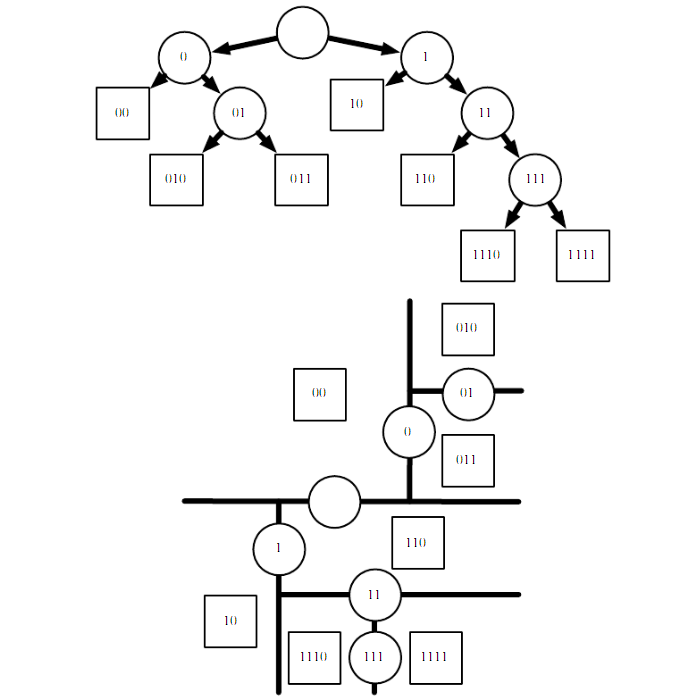
\includegraphics[width=6in]{fig/chap5/5_7.png} 
   \caption{决策树的运作机理。(上图)树的每个节点选择将输入样本送至左子节点(0)或右子节点(1)。中间节点画作圆圈,叶子节点画作方块。每个节点都以二级制字符串表示其在树中的位置,在其父节点的识别编码后增补字节(0=左或上,1=右或下)。(下图)树将输入空间划分成不同区域。这个2D平面显示了决策树如何划分$R^{2}$,中间节点画在给样本分类的分割线上,叶子节点画在样本对应区域的中心。结果是一个分段等值函数,每个叶子节点都相当于一段。每个叶子节点都需要至少一个样本才能定义,所以决策树不能学习到局部最大值比样本数量还多的函数。}
   \label{fig:5_7}
\end{figure}

另有一类学习算法也将输入孔建分成了不同的区域,并且每个域自有独立的参数,这就是\textbf{决策树}(decision tree, Breiman et al.)及其变种。如\ref{fig:5_7}所示,决策树的每个节点都对应输入空间里的不同区域,每个区域再被中间节点细分为子区域,并形成子节点(通常基于轴向切分)。空间由此继续细分为不重叠的区域,建立起叶子节点(leaf node)与输入区域(input region)之间的一一对应。每个叶子节点通常将来自同一输入区域的点映射到相同的输出。

决策树一般通过特殊的算法训练,这些算法超出了本书的范畴。如果一个学习算法可以学习任意规模的树,那么我们就可以认为该算法是无参数的,尽管在实际应用中决策树通常都经过基于规模限制的正则化(regularization)以转换为有参数模型。

决策树在使用中经常经过轴向切分(axis-aligned split),每个节点对应一个不变的输出,很多逻辑回归都能轻易解决的问题对决策树却可能很困难。例如,如果我们有一个二分类问题,当$x_{2} > x_{1}$时为正类,那么决策边界可能就不是轴向的。于是决策树就需要结合多个节点来估测决策边界,估测过程是调用一个阶跃函数(step function)在正确的决策函数边界上做等值、轴向的反复走步。

如前所述,近邻预测器和决策树存在很多限制,然而当计算资源有限的时候它们还是非常实用的。通过思考更复杂的高级算法与k近邻、决策树之间的相似与差异,我们可以获得发现更精巧算法的直觉。

关于传统监督学习算法的材料,可查看Murphy(2012), Bishop(2006), Hastie et al.(2001)或者其他机器学习课本。

\section{非监督学习算法}
\label{sec:5.8}

前承\ref{sec:5.1.3}节,无监督算法只有“特征”而没有监督信号。监督算法和非监督算法之间并没有明确严苛的区别,因为一个值属于特征还是监督者提供的标签,这本来也不存在客观定义。一般来讲,无监督学习指的是那些不借助人为干预或外部信息,直接从分布中提取信息的算法。与其高度相关的概念有:密度估计,样例提取,降噪,流形,聚类等。

有个经典的无监督学习任务,就是寻找数据的“最佳”表征。这里的“最佳”指的是尽可能多的保留$x$的信息,同时保证表征的形式比$x$本身更加简单。

定义更简单的表征可以有多种方式。三种最常见的是低维表征(low-dimensional representation)、稀疏表征(sparse representation)和独立(independent representation)表征。低维表征试图尽量压缩信息;稀疏表征(Barlow, 1989;Olshausen and Field, 1996;Hinton and Ghahramani, 1997)将数据集嵌入到另一个主要由0构成的表征里。使用稀疏表征往往要升维,整体结构是将数据分发至表征空间的各个轴上;独立表征则试图理清数据变化背后的来源,以使表征的每个维度之间都服从统计独立。

当然这三个标准并非互斥关系。低维表征常常降低元素之间的依赖性,这是因为压缩信息量的一种常用方法就是识别并剔除数据中的冗余关系。冗余的降低让降维算法可以直接忽略少部分信息以达到更大的压缩程度。

表征(representation)是深度学习的核心命题,也是本书的核心命题。在这一节中,我们开发了几个表征学习的例子,这些示例算法将展示如何实现上面所有的三个判据。之后的章节也将介绍更多从不同角度演绎这三大判据的表征学习算法以及其他判据。

\subsection{主成分分析}
\label{sec:5.8.1}

在\ref{sec:2.12}中,我们已经了解到,主成分分析(PCA, principal component analysis)算法提供了一种压缩数据的方法。我们同样把PCA看作是一种无监督学习算法,它从数据中学习表征,这样的表征基于以上提到的两种判据。PCA学习维数低于初始输入的表征,也学习一个元素与其他元素线性无关的表征。这正是统计独立表征学习的第一步。为了获得完全的独立性,表征学习算法必须将变量之间的非线性关系也识别并剔除掉。

\begin{figure}[htbp]
   \centering
   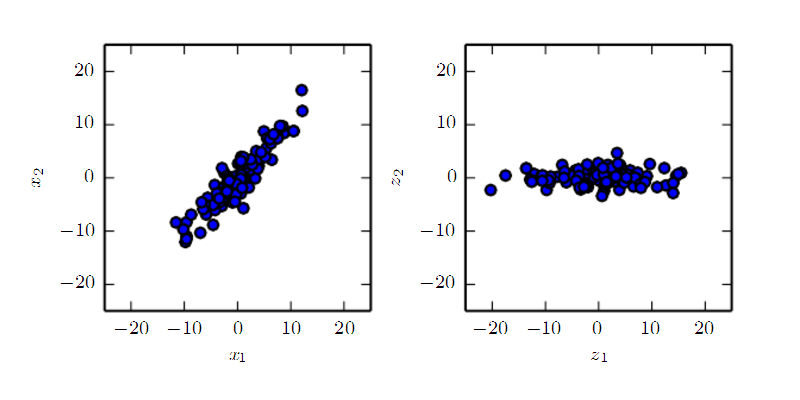
\includegraphics[width=6in]{fig/chap5/5_8.png} 
   \caption{PCA学习一种线性投影方式,使变化最大的方向与新空间的轴平行。(左图)初始数据由样本$x$构成,在这一空间中,数据的变化可能与坐标轴不平行。(右图)经过变换的数据$z=x^{T}W$现在基上是沿着轴$z_1$变化。第二大的变化方向则沿着$z_2$.}
   \label{fig:5_8}
\end{figure}

PCA学习数据的正交线性变换,将输入$x$投影到表征$z$,如\ref{fig:5_8}所示。在\ref{sec:2.12}中已经介绍过,我们可以学习构建原始数据的“最佳”一维表征(最小二乘法),这一表征其实就对应数据的第一个主成分。接着我们可以把PCA用作一种简单有效的降维方法来尽可能多的保留数据中的信息(同样根据最小二乘法)。接下来,我们将学习PCA表征如何与原始数据表征\textit{X}“去相关”。

考虑一个$m\times n$的设计矩阵$X$。假设数据的平均值为0,$E[x]=0$。如果非零,只需在预处理中将所有数据同时减去现有均值即可。

$X$的无偏协方差矩阵写作:
\begin{equation}
	Var[x] = \frac{1}{m-1}X^{T}X
   \label{form:5.85}
\end{equation}

PCA找到一个表征(通过线性变换)$z=x^{T}W$使$Var[z]$为对角阵。
在\ref{sec:2.12}中,我们已知设计矩阵$X$的主成分由$X^{T}X$的特征向量给出:
\begin{equation}
	X^{T}X = W\Lambda W^{T}
   \label{form:5.86}
\end{equation}

本节,我们将挖掘另一种主成分的推导方法。主成分也可以由奇异值分解(SVD)得到。特别地,他们就是$X$的右奇异向量。为证此理,设$W$为分解$X=U\Sigma W^{T}$的右奇异向量。再将$W$的原始特征向量还原为特征向量基。
\begin{equation}
	X^{T}X = (U\Sigma W^{T})^{T} U\Sigma W^{T} = W\Sigma^{2}W^{T}
   \label{form:5.87}
\end{equation}

SVD可以帮助我们证明PCA可以得到对角的$Var[z]$。对$X$做SVD,我们可以将$X$的方差写作:
\begin{align}
	Var[x] & = \frac{1}{m-1}X^{T}X\\
	&= \frac{1}{m-1}(U\Sigma W^T)^T U\Sigma W^T\\
	&=\frac{1}{m-1}W\Sigma ^T U^T U \Sigma W^T\\
	&=\frac{1}{m-1}W \Sigma ^2 W^T\\
\end{align}

上面的推导中我们用到了$U^T U = I$因为奇异值分解的矩阵$U$被定义为正交矩阵。下面证明如果我们取$z=x^T W$,可以确定$z$的协方差是对角矩阵:
\begin{align}
	Var[x] & = \frac{1}{m-1}Z^{T}Z\\
	&= \frac{1}{m-1}W^T X^T X W\\
	&=\frac{1}{m-1}W^T W \Sigma ^2 W W^T\\
	&=\frac{1}{m-1}\Sigma ^2\\
\end{align}
这次我们利用了$W^T W = I$,同样来自SVD的定义。

以上分析展示了当我们通过线性变换$W$将数据$x$投影到$z$的时候,所生成的表征拥有对角协方差矩阵($\Sigma ^2$),也就说明了$z$的每个元素都是相互独立的。

将数据变换成为元素相互独立的表征,这种能力是PCA的重要属性,也展现了表征的作用在于试图理清数据背后未知的变化因子。在PCA当中,这种理顺工作的形式是旋转输入空间使变化的主轴与新的表征空间$z$的基向量平行。

相关性(correlation)是数据元素之间依赖性(dependency)的重要组成部分,我们也同样对表征学习如何理顺更复杂的特征依赖感兴趣。为此,除了简单的线性变换,我们还有更多工作要做。

\subsection{k平均聚类}
\label{sec:5.8.2}

另一个简单的表征学习实例是k平均聚类(k-means clustering)。k平均算法将训练集分为k个组,每个组内部的样本相互都很接近。我们可以进一步认为该算法提供了一个k维的o独热码向量$h$来表征输入$x$。如果$x$属于一个类$i$,则$h_i=1$且$h$的其他元均为0。

k平均聚类提供的独热码正是稀疏表征的一个实例,因为每个输入的绝大多数元都是0。之后我们会接触到其他算法,它们能够学习更灵活的稀疏表征——每个输入不止有一个元为1。独热码是稀疏矩阵的极端情况,因为它丢失了分布表征的很多优点。但同时独热码也赋予了算法统计上的优势(天然地表达出同类样本相互接近)而且也带来了计算优势,整个表征可由一个整数代表。

k平均算法



\section{随机梯度下降法}
\label{sec:5.9}

\section{构建机器学习算法}
\label{sec:5.10}

\section{深度学习算法的动力}
\label{sec:5.11}
\part{深度学习:实战}
\label{part:2}

本部分将介绍可以用于解决实际问题的现代深度学习方法。


深度学习拥有着漫长历史和许多的应用,一些尝试至今已硕果累累。一些看起来野心十足的目标已经变为现实。深度学习中仍需探索的分支我们将留到最后一部分进行介绍。


本部分只介绍那些在工业中进行应用实践并获得成功的方法。


现代深度学习为有监督学习提供了一个十分强大的框架。通过增加层数或层间的单元数,网络可模拟更为复杂的函数。许多任务中都有把一个向量映射到另一个向量的工作,人类对这类工作翻译十分迅速,如果给出足够大的模型和大量的标签数据,深度学习也可以很好的完成这项工作。另外那些非向量映射可以描述的困难工作,甚至人类都需要时间思考和反应的,目前是不在深度学习讨论的范畴内。


本部分将讨论参数方程近似技术,这几乎要被所有的现代深度学习实践所使用。我们先介绍用于描述这些方程的前馈深度网络模型,然后我们会介绍正则化和优化等进一步的技术。缩放这些模型,使之适应于高分辨率的图像和长时间序列则需要进一步的讲述。我们将会介绍可用于缩放图像的卷积网络和处理时间序列的循环神经网络。最后,我们将总结一些可用于具体实践的指导,包括设计、构建、配置深度学习等,并对一些深度学习应用进行回顾。


本部分的章节对实践者来说最为重要,实践者们将开始使用深度学习技术解决真实世界中的问题。

\chapter{深度前馈网络}
\label{chap:6}
%%%%%%%%%%%%%%%%%%%%%%%%%%%%%%%%%%%%%%%%%%%%%%%%%%%%%%%%%
%%%%%%%%%%%%%%%%%% author:jim1949@163.com %%%%%%%%%%%%%%%
%%%%%%%%%%%%%%%%%% part:6.0-6.2           %%%%%%%%%%%%%%%
%%%%%%%%%%%%%%%%%%%%%%%%%%%%%%%%%%%%%%%%%%%%%%%%%%%%%%%%%

\emph{深度前馈网络}又被称为\emph{前馈神经网络}或\emph{多层感知机},是一种深度学习模型。前馈神经网络的目标是近似一个函数$f^*$。比如对于一个分类器来说,$y=f^*(\textbf{x})$ 把输入$\textbf{x}$映射到类别$y$。前馈网络定义了这个映射$\textbf{y}=f(\textbf{x};\bm{\theta})$,并且通过学习参数$\bm{\theta}$来近似真实的映射。


这类模型被称为\emph{前馈}是因为信息通过输入$\textbf{x}$流向用于定义函数$f$的中间计算,最后流向输出$\textbf{y}$。网络中并没有从输出流入模型的\emph{反馈}连接。当前馈网络扩展至包含反馈的连接时,就会被称为第\ref{chap:10}章中介绍的\emph{循环网络}。


前馈网络对机器学习的实践者非常重要。它组成了许多重要商业应用的基础模块。比如,用于照片中物体识别的卷积网络就是一种特化的前馈网络。前馈网络也是通往循环网络的重要踏脚石,而循环网络支撑了许多自然语言相关的应用。


前馈神经网络之所以被称为\emph{网络}是因为它非常典型的是由许多不同的函数组成的。这些函数的组成方式可以由一个有向无环图来描述。例如,函数$f(\textbf{x})=f^{(3)}(f^{(2)}(f^{(1)}(\textbf{x})))$可以由$f^{(1)}$、$f^{(2)}$、$f^{(3)}$链式的串联组成,而链式结构是神经网络中最常用的结构。在这个情况中,$f^{(1)}$被称为网络的\emph{第一层},$f^{(2)}$被称为网络的\emph{第二层},以此类推。这个链的长度就定义了网络的深度。前馈网络的最后的一层被称为\emph{输出层}。在神经网络的训练过程中,我们不断使得$f(\textbf{x})$近似于$f^*(\textbf{x})$。在不同的训练节点上,训练数据提供了关于$f^*(\bm{x})$的带有噪声、近似的样本。每个样本$\bm{x}$都有一个使得$y \approx f^*(\bm{x})$的标签。训练数据指定了在每个$\bm{x}$上输出层的直接表现,但没有直接指定其他层的行为。学习算法需要决定如何使用这些层来产生相应的输出,但训练数据并未指定每一层需要做什么。所以学习算法需要知道如何使用这些层来对$f^*$进行最优的近似,因为训练数据并不会为每一层都指定输出,这些没被指定输出的层就被称为\emph{隐层}。


最终,这些网络被称为\emph{神经},因为它们是由神经科学启发而来的。网络的每个隐层都是典型的向量值,隐层的维度决定了模型的\textbf{宽度}。这些向量中的每一个值都可以被看做对一个神经元的模拟。与其把这些层当做是向量间的映射函数,不如把每一层当做由许多并行的\emph{单元}组成,而每个单元代表着一个向量到标量的映射函数。每个单元在这个场景下都被当做一个神经元,它从其他的单元中获取输入并计算自己的激活值。这种使用向量来代表网络层的想法来自于神经科学。$f^{(i)}(\bm{x})$的计算行为也是或多或少来自于对生物神经元计算行为的观察。然而,现代的神经网络研究也
受了许多数学和工程的指导,而且其目的也并非是完美的模拟大脑。我们最好把前馈网络当初一种函数近似技术,用于达到统计上的概括,偶尔会借鉴一些我们对大脑的先验知识,而非用于对大脑进行建模。



对前馈网络进行了解的一种方法是先从线性模型开始,并考虑如何突破线性模型的限制。如逻辑回归和线性回归等线性模型非常吸引人,因为他们是封闭形式的或可以进行凸优化,可以非常有效和可靠的进行拟合。但线性模型也有个显著的缺点,它们只能拟合线性函数,因此线性模型不能理解两个输入变量之间的相互作用。


为了使得线性模型可以表达$\bm{x}$的非线性函数,我们可以把输入转换为$\phi(\bm{x})$,$\phi$是一个非线性转换。等效的,我们也可以用\ref{sec:5.7.2}章中提到的核方法,通过应用$\phi$的映射来获得非线性的学习算法。我们可以认为$\phi$提供了一组可以描述$\bm{x}$的特征,或认为提供了$\bm{x}$的新的形式。


问题在于,我们如何选择映射$\phi$。

\begin{enumerate}
 	\item 一个选择是使用通用的$\phi$, 比如RBF核用的无限维的$\phi$。如果$\phi(\bm{x})$的维度足够高,总能有办法来拟合训练集,但测试集上的泛化缺是个问题。通用化的特征映射通常只基于局部平滑的原则,并没有编码进足够的先验信息来进一步解决问题。
	\item 另一个选择是手工的$\phi$。在深度学习来临之前,这是一个主流方案。这个方法对每个不同任务都耗费数十年的人力,并需要实践者在不同的领域如语音识别或计算机视觉进行特化,且领域之间的共同点非常少。
	\item 深度学习的策略则是学习$\phi$。在这个方法中,模型是$y=f(\bm{x};\bm{\theta},\bm{w}) = \phi(\bm{x};\bm{\theta})^T\bm{w}$。参数$\theta$可以用于从许多的函数中学习到想要的$\phi$,参数$\bm{w}$用于控制$\phi(\bm{x})$到指定的输出。这是一个深度前馈网络的示例,$\phi$是其隐层。这个方法是三个中唯一放弃了训练问题的凸性质的,但其优点远胜于缺点。在这个方法把输入转换后的形式记为$\phi(\bm{x};\bm{\theta})$,使用优化算法来找到使得转换后的性质最优的$\theta$。通过提供一个非常广阔的$\phi(\bm{x};\bm{\theta})$族,我们可以让这个方法像第一个方法一样具有高通用性。它也具有第二个选择的优势。人可以通过设计$\phi(\bm{x};\bm{\theta})$族来编码自身的知识,并帮助泛化。其优势是人类设计者只需要找到正确的函数簇而非找到唯一的正确的函数。
\end{enumerate}


通过学习特征来提高模型性质的准则超出了本章前馈网络的讨论范围。但这是深度学习的主题,可以适用于本书描述的任何模型。前馈网络的原则是学习从$\bm{x}$到$\bm{y}$的确定性映射,并且不引入反馈连接。后面介绍的一些模型会使用这些原则来学习统计性映射,学习带反馈的函数,或学习在一个向量上的概率分布。


我们以一个简单的反馈网络示例开始本章节。然后,我们解决部署前馈网络所需的设计决策。首先,训练前馈网络需要很多和设计线性模型一样的设计决策:选择优化器、损失函数、输出单元的形式。我们先回顾基于梯度学习的基本知识,然后再看一些前馈网络独有的设计决策。
%%%%%%%%%%%%%%%%%%%%%%%%%%%%%%%%%%%%%%%%%%%%%%%%%%%%%%%%%
%%%%%%%%%%%%%%%%%%% author:liviclee %%%%%%%%%%%%%%%%%%%%%
%%%%%%%%%%%%%%%%%%% part:6.3-6.7    %%%%%%%%%%%%%%%%%%%%%
%%%%%%%%%%%%%%%%%%%%%%%%%%%%%%%%%%%%%%%%%%%%%%%%%%%%%%%%%

\section{隐藏单元}
\label{sec:6.3}

\section{架构设计}
\label{sec:6.4}

\section{反向传播及其他微分算法}
\label{sec:6.5}

\section{前馈神经网络的发展史}
\label{sec:6.6}

\chapter{深度学习的正则化}
\label{chap:7}
%%%%%%%%%%%%%%%%%%%%%%%%%%%%%%%%%%%%%%%%%%%%%%%%%%%%%%%%%
%%%%%%%%%%%%%%%%%% author:ysh329 %%%%%%%%%%%%%%%%%%%%%%%%
%%%%%%%%%%%%%%%%%%%%%%%%%%%%%%%%%%%%%%%%%%%%%%%%%%%%%%%%%
\chapter{训练深度模型的优化方法}
\label{chap:8}
%%%%%%%%%%%%%%%%%%%%%%%%%%%%%%%%%%%%%%%%%%%%%%%%%%%%%%%%%
%%%%%%%%%%%%%%%%%%% author:wzwei1636@163.com  %%%%%%%%%%%
%%%%%%%%%%%%%%%%%%% part:8.0-8.2              %%%%%%%%%%%
%%%%%%%%%%%%%%%%%%%%%%%%%%%%%%%%%%%%%%%%%%%%%%%%%%%%%%%%%
\section{8.0}
%%%%%%%%%%%%%%%%%%%%%%%%%%%%%%%%%%%%%%%%%%%%%%%%%%%%%%%%%
%%%%%%%%%%%%%%%%%%% author:SilentSkyWalker %%%%%%%%%%%%%%
%%%%%%%%%%%%%%%%%%% part:8.3-8.5           %%%%%%%%%%%%%%
%%%%%%%%%%%%%%%%%%%%%%%%%%%%%%%%%%%%%%%%%%%%%%%%%%%%%%%%%

\section{8.3}
%%%%%%%%%%%%%%%%%%%%%%%%%%%%%%%%%%%%%%%%%%%%%%%%%%%%%%%%%
%%%%%%%%%%%%%%%%%%% author:dimitri0802 %%%%%%%%%%%%%%%%%%
%%%%%%%%%%%%%%%%%%% part:8.6-8.7       %%%%%%%%%%%%%%%%%%
%%%%%%%%%%%%%%%%%%%%%%%%%%%%%%%%%%%%%%%%%%%%%%%%%%%%%%%%%

\section{8.6}
\chapter{卷积网络}
\label{chap:9}
%%%%%%%%%%%%%%%%%%%%%%%%%%%%%%%%%%%%%%%%%%%%%%%%%%%%%%%%%
%%%%%%%%%%%%%%%%%%% author:ifighting %%%%%%%%%%%%%%%%%%%%
%%%%%%%%%%%%%%%%%%% part:9.1-9.6     %%%%%%%%%%%%%%%%%%%%
%%%%%%%%%%%%%%%%%%%%%%%%%%%%%%%%%%%%%%%%%%%%%%%%%%%%%%%%%
\section{9.1}
\label{sec:9.1}
\section{9.2}
\label{sec:9.2}
\section{9.3}
\label{sec:9.3}
\section{9.4}
\label{sec:9.4}
\section{9.5}
\label{sec:9.5}
%%%%%%%%%%%%%%%%%%%%%%%%%%%%%%%%%%%%%%%%%%%%%%%%%%%%%%%%%
%%%%%%%%%%%%%%%%%%% author: iWeisskohl %%%%%%%%%%%%%%%%%%
%%%%%%%%%%%%%%%%%%% part:9.7-9.11      %%%%%%%%%%%%%%%%%%
%%%%%%%%%%%%%%%%%%%%%%%%%%%%%%%%%%%%%%%%%%%%%%%%%%%%%%%%%

\section{9.6}
\label{sec:9.6}
%%%%%%%%%%%%%%%%%%%%%%%%%%%%%%%%%%%%%%%%%%%%%%%%%%%%%%%%%
%%%%%%%%%%%%%%%%% author:dormir_yin %%%%%%%%%%%%%%%%%%%%%%%%%%%%%%
%%%%%%%%%%%%%%%%%%%%%%%%%%%%%%%%%%%%%%%%%%%%%%%%%%%%%%%%%

\chapter{序列模型:循环网络与递归网络}
\label{chap:10}
递归神经网络
%%%%%%%%%%%%%%%%%%%%%%%%%%%%%%%%%%%%%%%%%%%%%%%%%%%%%%%%%
%%%%%%%%%%%%%%%%%%%author:rickymf4%%%%%%%%%%%%%%%%%%%%%%%
%%%%%%%%%%%%%%%%%%%%%%%%%%%%%%%%%%%%%%%%%%%%%%%%%%%%%%%%%
\chapter{实战方法}
\label{chap:11}

成功地应用深度学习技术远远不仅仅需要知道有哪些算法和这些算法的原理。一个好的机器学习实践者亦需要知道如何针对特定的应用选择算法,如何监控实验并对获得的反馈做出回应,从而优化该机器学习系统。在机器学习系统的日常开发中,实践者们需要决定是否需要搜集更多的数据,是增加还是减少模型的容量,是加上还是去掉规则化特征,是改进模型的优化,还是改进模型中的近似推理,亦或是对模型的实现程序进行调试。所有这些操作都是非常耗时的尝试,所以能够确定正确的行动方针是很重要的,而不是盲目猜测它。

这本书的大部分内容是关于各种机器学习模型、训练算法,和目标函数。这可能会造成这样的印象:成为机器学习专家最重要的本领是要了解各种机器学习技术并擅长不同类型的数学。 然而在实践中,正确地使用一个常见的算法比草率地使用一个晦涩的算法要好。算法的正确应用取决于掌握一些相当简单的方法。本章节中许多建议改编自\cite{Ng ( 2015 )}.

我们建议如下的实际设计过程:
\begin{itemize}
\item 确定您的目标 - 要使用的误度量和相应的目标价值。这些目标和误差度量应该由应用要解决的问题来驱动。
\item 尽快建立一个可以工作的端到端的流水线,包括适当估计它的性能指标。
\item 较好地给系统装上仪表来确定其性能瓶颈。诊断哪些组件的性能低于预期,以及是否是由于过度拟合、欠拟合,或数据或程序中存在着缺陷。
\item 基于来自仪表中特定的发现,重复地进行增量变更,如收集新数据,调整超参或更改算法。
\end{itemize}

我们将采用街景地址号码翻译系统作为一个运行的例子 (\cite{ Goodfellow et al. , 2014d })。 这个应用的目的是将建筑添加到谷歌地图中。街景车对建筑进行拍摄并记录照片对应的GPS坐标。通过卷积网络来识别每张照片中的地址号码,使得谷歌地图数据库可以将该地址加入到正确的位置上。关于如何开发这个商业应用程序的故事给出了如何遵循我们倡导的设计方法的例子。我们现在来描述这个过程中的每个步骤。

\section{性能指标}

确定目标(根据将采用的错误率指标)是必要的第一步,因为你的错误率指标将指导你以后的所有操作。你还应该知道你想要什么级别的性能。

请记住,对于大多数应用,不可能实现绝对零错误率。即使你有无限训练数据,并且可以恢复真实的概率分布,而贝叶斯误差定义了你可以希望实现的最小错误率。这是因为你的输入特征可能不包含有关输出变量的完整信息,或者因为系统可能是内在随机的。你也将受限于有限数量的训练数据。

由于各种原因,训练数据的量被限制了。当你的目标是构建一个一流的实际的产品或服务时,您通常可以收集更多数据,但必须确定进一步减少错误率的价值,并将其与收集更多数据的成本进行权衡。数据收集可能需要时间、金钱或使人遭受痛苦(例如,如果您的数据收集过程涉及侵入性的医学测试)。 而当你的目标是回答在固定的基准上哪个算法的表现更好时,通常是不允许收集更多数据作为基准的训练集的。

如何给性能水平确定一个合理的期望?通常,在做学术时,我们基于以前发布的基准测试结果,可以做一些错误率的估计。而在做实际项目时,我们考虑的错误率是要让我们的应用是安全的,成本效益的,或是吸引消费者的。一旦确定了实际期望的错误率,你的设计决策将以达到此错误率为指导。


%%%%%%%%%%%%%%%%%%%%%%%%%%%%%%%%%%%%%%%%%%%%%%%%%%%%%%%%%
%%%%%%%%%%%%%%%%%%%author:MalcolmSun%%%%%%%%%%%%%%%%%%%%%
%%%%%%%%%%%%%%%%%%%%%%%%%%%%%%%%%%%%%%%%%%%%%%%%%%%%%%%%%

\chapter{应用}
\label{chap:12}


\subsection{12.1.2}
\label{sec:12.1.2}

\section{12.3}
\label{sec:12.3}
%%%%%%%%%%%%%%%%%%%%%%%%%%%%%%%%%%%%%%%%%%%%%%%%%%%%%%%%%
%%%%%%%%%%%%%%%%%% author:chaocraig %%%%%%%%%%%%%%%%%%%%%
%%%%%%%%%%%%%%%%%% part:12.4-12.6   %%%%%%%%%%%%%%%%%%%%%
%%%%%%%%%%%%%%%%%%%%%%%%%%%%%%%%%%%%%%%%%%%%%%%%%%%%%%%%%


\section{自然語言處理}{12.4}

自然語言處理(NLP)是電腦使用人類的語言,包括英語或法語等。特殊設計的计算机程序通常读取和发出专门的语言,目的在允许通过简单的程序进行高效和明确的解析。

Natural language processing (NLP) is the use of human languages, such as English or French, by a computer. Computer programs typically read and emit specialized languages designed to allow efficient and unambiguous parsing by simple programs. More naturally occurring languages are often ambiguous and defy formal description. Natural language processing includes applications such as machine translation, in which the learner must read a sentence in one human language and emit an equivalent sentence in another human language. Many NLP applications are based on language models that define a probability distribution over sequences of words, characters or bytes in a natural language.






\part{深度学习研究}
\label{part:3}

\chapter{线性模型}
\label{chap:13}

%%%%%%%%%%%%%%%%%%%%%%%%%%%%%%%%%%%%%%%%%%%%%%%%%%%%%%%%%
%%%%%%%%%%%%%%%%%%%author:shanong%%%%%%%%%%%%%%%%%%%%%%%%
%%%%%%%%%%%%%%%%%%%%%%%%%%%%%%%%%%%%%%%%%%%%%%%%%%%%%%%%%
    深度学习的很多前沿研究都是围绕着建立一个输入变量的概率模型,如Pmdoe(x).原则上,这样的模型可以根据环境提供变量使用概率去推算预测任何变量。这类模型也用潜变量(latent variables)h,如Pmodel(x) = Ehpmodel(x | h)。这些潜变量提供了另一种表示数据的方法。基于潜变量分布式表达 跟
%%%%%%%%%%%%%%%%%%%%%%%%%%%%%%%%%%%%%%%%%%%%%%%%%%%%%%%%%
%%%%%%%%%%%%%%%%%%% author:hijeffery %%%%%%%%%%%%%%%%%%%%
%%%%%%%%%%%%%%%%%%% part:14.0-14.6   %%%%%%%%%%%%%%%%%%%%
%%%%%%%%%%%%%%%%%%%%%%%%%%%%%%%%%%%%%%%%%%%%%%%%%%%%%%%%%

\chapter{自编码器}
\label{chap:14}

\emph{自编码器}是神经网络的一种,用以训练来实现将输入复制到输出的目的。在其内部,有一个用编码表示输入的隐层$h$。自编码器可以看作由两部分组成:编码函数$h = f(x)$ 和进行信号重建的解码函数$r = g(h)$。 具体结构如图\ref{fig:14.1}所示。如果自编码器学到的结果仅仅是处处将$g(f(x)) = x$,则其没有起到任何作用。相反,自编码器被设计成了不能够完美的复制输入到输出的工作方式。通常他们被限定在只能够近似的复制,并且只复制能够与训练数据相像的输入。鉴于模型被强制执行输入的某些部分应当被复制,所以通常来讲,自编码器能够学习到数据的有用的特性。
\begin{figure}[htbp] %  figure placement: here, top, bottom, or page
   \centering
   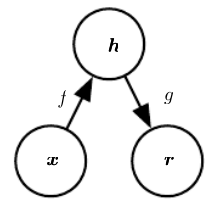
\includegraphics[width=1in]{fig/chap14/14_1.png} 
   \caption{自编码器的基本结构,将输入信号$x$通过一个内部表征或者编码$h$ 映射到输出(也叫重建) $r$。 自编码器有两个子部分:编码器(将$x$映射到$h$)与解码器(将$h$映射到$r$)。}
   \label{fig:14.1}
\end{figure}

现代自编码器已经从执行特定的函数映射扩展到了执行随机映射$p_{encoder}(h|x)$ 和 $p_{decoder}(x|h)$。

自编码器的思想已经在神经网络研究领域存在了几十年。传统上来讲,自编码器是用来执行数据降维与特征学习的。近来,自编码器与隐变量模型的联系使得自编码器成为生成模型的研究前沿,详情见本书第\ref{chap:20}章介绍。自编码器可以视为前馈网络的一种特殊形式,并且可以用与其相同的方式进行训练,如以子集沿着反向传播计算的梯度下降方向求解。同一般的前馈网络不同的是,自编码器也可以用\emph{再循环}的方式进行训练,即对比原始输入的网络相应与重建信号作为输入的网络相应的差别。再循环技术被视为比反向传播算法更为接近生物特性的方法,但是其很少被出现在其他机器学习应用中。

\section{不完备自编码器}
\label{sec:14.1}
将输入复制到输出听起来似乎无特别作用,但其实我们也不关心解码器的输出。事实上,我们期望通过训练自编码器实现复制输入的任务能够产生有实用意义的$h$。

一个从自编码器获取有效的特征的方法是将$h$限定到一个比$x$更低的维度上。特征维度比输入维度低的自编码器是\emph{不完备}的。学习一个不完备的特征迫使自编码器捕获到训练数据中的最为突出的特征信息。

学习过程可以简单的表述为最小化一个随时函数的形式:
\begin{equation}
	L(x,g(f(x)))
\end{equation}
其中,损失函数 $L$ 通过如最小化均方误差等限定$g(f(x))$ 与 $x$ 尽量相近。 

当解码器是线性函数,并且$L$ 是均方误差时,不完备自编码器学习到的生成子空间与PCA一致。此时,被用来执行复制任务的自编码器事实上附加学到了训练数据的主子空间。

因此,具有非线性编码函数$f$和非线性解码函数$g$的自编码器可以学习到更强有力的非线性泛化PCA。遗憾的是,如果编码与解码部分被给予太强能力的化,自编码器仍然仅仅完成复制输入到输出的功能而忽略了抽取数据分布等有效信息的能力。理论上说,我们可以设想一个只有一维编码的自编码器,其编码器具有强大的能力将每一个训练数据$x^{(i)}$表示成编码$i$。此外,解码器能够学习并将每一个整型值映射回特定的训练数值上。这种特殊情形在现实中不会出现,但其足够说明,一个被训练用来进行数据复制的自编码器,如果被赋予了过与强大的能力,并不会学习到任何与用的信息。

\section{正则化自编码器}
\label{sec:14.2}
编码维数比输入维数低的自编码器能够学习到数据分布的最为显著的信息。我们也提到,如果编码与解码部分被赋予了太强的能力,会导致自编码器学习不到任何有用的东西。

相似的问题也会发生在编码维数同输入维数相同的自编码器中,以及隐层编码维数比输入数据维数大的\emph{过完备}自编码器中。在这种情况时,甚至线性的编码器与解码器也会产生直接复制输入数据到输出数据而不获取任何数据分布有效信息的问题。

理想来说,我们只要根据待建模分布的复杂度选取编码的维数以及编码器解码器的容量,我们就可以成功的训练任何结构的自编码器。正则化自编码器就提供了这种功能。正则化自编码器不是通过控制编码器解码器的层数与编码长度来达到限定模型容量的目的,而是通过损失函数来促使模型具有复制输入到输出以外的特性的。这些特性包括描述特征的稀疏度,缩小特征的偏导数以及对于噪声和数据确实的鲁棒性等。正则化自编码器可以是非线性的或者过完备的,但是,即便有足够容量可以取巧只学习简单的复制函数,其仍可以学习到数据分布的一些有用的东西。

除了本处列举的几个可以被很自然的理解为正则化自编码器的方法之外,几乎任何有隐变量以及推理过程(从给定输入推算隐变量表示)的生成模型都可以被视为一种具有特殊形式的自编码器。有两种同自编码器有此种高度关联的生成模型如变分自编码器和随机生成网络,他们都是Helmholtz机的子类。这些模型会自然的学习高容量,过完备的编码方式,并且不需要归一化处理才能使这些编码具有实用性。这些编码之所以有效,是因为模型是被训练来近似最大化训练数据的概率分布,而不是去执行复制输入输出的操作。

\subsection{稀疏自编码器}
\label{sec:14.2.1}
稀疏自编码器是在自编码器的基础上,简单的引入稀疏惩罚项$\Omega(h)$加到编码层上,并同重建误差项一起训练:
\begin{equation}
L(x,g(f(x))) + \Omega(h) 
\end{equation}
其中,$g(h)$ 是解码器的输出,并且通常编码器的输出为$h = f(x)$。

稀稀疏自编码器通常被用于其他任务中,如分类。稀疏泛化的自编码器必须能够对其针对的训练数据的特定统计特性做出响应,而不能是简单的复制操作。此时,训练执行复制任务,并且有一定的稀疏惩罚项能够得到具有附加特征表示能力的模型。

我们可以把惩罚项$\Omega(h)$ 简单的看作添加到前馈网络上的正则项,该网络主要是实现复制输入到输出的任务(非监督学习目标函数),或者根据这些稀疏特征执行一些有监督的任务(监督学习目标函数)。
同其他正则项如权值衰减等不同,改该正则项并没有直观的贝叶斯解释。如\ref{sec:5.6.1}中所描述,包含权值衰减和其他正则化惩罚项的训练过程可以被视为贝叶斯推断的最大后验近似,其中加入的正则惩罚项可以视为参数模型的先验概率。在这个角度,最大化的最大似然同最大化$p(\theta|x)$相关,有等效于最大化$log p(x|\theta) + log p(\theta)$。$log p(x|\theta)$是常规的数据对数似然项,对数先验项$log p(\theta)$包含对于$\theta$的某些特定值的偏好。这部分内容在第\ref{sec:5.6}节中有介绍。正则化自编码器则不赞同这种解释,因为正则项本身依赖于数据,因此语义上来讲,其定义并不是严格的先验。

与其将稀疏惩罚项视为复制任务的正则项,我们不妨将整个稀疏自编码框架看过是有隐变量的生成模型最大似然训练。假设我们有一个模型,其观测变量为$\bm{x}$隐变量为$\bm{h}$,并且其联合概率分布为$p_{model}(\bm{x},\bm{h}) = p_{model}(\bm{x}|\bm{h})$。我们定义$p_{model}(\bm{h})$为模型对于隐变量的先验概率,表示模型在观察变量$\bm{x}$前的置信度。同我们之前使用“先验”这个词有些不同,这里是指,在我们观察到训练数据之前,$p(\bm{\theta})$ 代表了我们对于模型参数的置信度。其对数似然可以分解为
\begin{equation}
	log p_{model}(\bm{x}) = log \sum_{\bm{h}}p_{model}(\bm{h},\bm{x})
\end{equation}
自编码器可以视为用$\bm{h}$的一个最相似的点对上述求和的近似。这同稀疏表示生成模型(\ref{sec:13.4}节)很像,但$\bm{h}$是参数化编码器的输出而不是推测最相似$\bm{sh}$的优化结果。从这个角度,给定$\bm{h}$后,须最大化
\begin{equation}
	log p_{model}(\bm{h},\bm{x}) = log p_{model}(\bm{h}) + log p_{model}(\bm{x}|\bm{h})
\end{equation}
其中,$log p_{model}(\bm{h})$ 可以是稀疏诱导项。比如,拉普拉斯先验,
\begin{equation}
	p_{model}(h_i) = \frac{\lambda}{2}e^{- \lambda |h_i|},
\end{equation}
对应着一个绝对值的稀疏惩罚项。将对数先验表示为绝对值惩罚项,则
\begin{equation}
	\Omega(\bm{h}) = \lambda \sum_i | h_i |
\end{equation}
\begin{equation}
	-log p_{model}(\bm(h)) = \sum_i (\lambda|h_i| - log \frac{\lambda}{2}) = \Omega(\bm{h}) + const
\end{equation}
其中,常数项只与$\lambda$有关,与$\bm{h}$无关。我们通常将$\lambda$视为超参数并忽略常数项,因为其对于参数学习没有影响。其他的先验函数如student-t分布,同样可以引入稀疏性。因为稀疏性是在用$p_{model}(\bm{h})$近似最大似然估计学习的过程中引入的,因此,从这个角度来看,稀疏惩罚项根本不能算作正则项。它仅仅是一系列模型隐变量分布的结果。这个思路给自编码器训练了一个不同的动机:其是训练生成模型的一个近似方法。同时,也给为什么自编码器学习到的特征有用提供了新的原因:他们描述了能够解释输入的隐变量。

稀疏自编码器的早期工作介绍了多种形式的稀疏,并提出了稀疏惩罚项同$log Z$之间的关系,$log Z$是在用最大似然估计无向图模型$p(x) = \frac{1}{Z}\hat{p}(x)$时产生的。其基本思路是,最小化$log Z$能够防止图模型在各处产生很高的概率,而对自编码器引入稀疏性能够防止在任意地方产生极低的重建误差。这种情况下,二者的联系存在于一个比较直观的普通机制理解层面上而不是仅仅有数学联系。在有向图模型$p_{model}(\bm{h}p_{model}(\bm{x}|\bm{h})$中,与稀疏项有关的$log p_{model}(\bm{h})$则具有更好的数学直观解释。

Glorot等人给出了一个实现稀疏(降噪)自编码器隐层编码$\bm{h}$中\emph{绝对零值}的方法。其思路是用ReLU来生成编码层。有了能够使描述逼近零值的先验(比如绝对值惩罚项),我们可以用间接的手段来控制特征表示中的零值的平均个数。

\subsection{降噪自编码器}
除了给损失函数添加惩罚项$\Omega$外,我们还可以通过改变损失函数项来实现训练自编码器学习有效信息的方法。

传统的自编码器的损失函数为
\begin{equation}
L(x,g(f(x)))
\end{equation}
其中,$L$是限定$g(f(x))$同 $x$相似度的损失函数,如对比二者的$L^2$ 范数损失。这使得$g\circ f$ 如果有能力的化就会学习到一个复制函数。

而\emph{降噪自编码器}则是最小化
\begin{equation}
L(x,g(f(\hat{x})))
\end{equation}
其中,$\hat{x}$是$x$ 被某种噪声干扰后的数据。降噪自编码器必须设法处理这种干扰而不是仅仅复制输入数据。

降噪训练的过程迫使$f$和$g$去学习潜在的$p_{data}(x)$的结构。降噪自编码器再次印证了在最小化重建误差的过程中,会有很多有用的性质作为副产品出现。
他们也可以作为过完备、高容量模型可以用来作为自编码器的例子,只要这些模型能够加入防止其学习到恒等函数的设计即可。      
降噪自编码器在第\ref{sec:14.5}节有更为详细的介绍。

\subsection{梯度惩罚正则化}
另一个正则化自编码器的方法是通过借用稀疏自编码器中的惩罚项$\Omega$, 
\begin{equation}
L(x,g(f(x))) + \Omega(h,x),
\end{equation}
但是,此处用了一个不同形式的$\Omega$
\begin{equation}
\Omega(h,x) = \lambda \sum_i \| \nabla_x h_i\|^2.
\end{equation}
这使得模型能够学到一个当$x$发生轻微变化的时候不会改变太多的函数。由于这个惩罚项仅仅作用于训练数据,其迫使自编码器能够捕获到训练数据的分布信息。

此种方式泛化的自编码器被成为\emph{收缩自编码器}。这种方法同降噪自编码器,流行学习以及概率模型具有很强的理论联系。更多的细节参看\ref{sec:14.7}节。

\section{表征能力,层级及深度}
\label{sec:14.3}
自编码器的训练通常只包含一层编码器和一层解码器。然而,这不是绝对的。事实上,用多层编码器和解码器能够提供非常多的好处。

我们可以回想第\ref{sec:6.4.1}节所述,用多层网络对于前馈型神经网络有很多的好处。因为自编码器是前馈型神经网络,这些优势也同样适用。此外,自编码器的编码器和解码器本身也都是前馈网络,所以这两部分都可以单独从网络深度获益。

网络深度的不平凡之处在于通用近似理论确保了对于有至少一层隐藏层的前馈神经网络,只要其具有足够的隐藏节点,就能够以任意精度近似任何函数(在一个很广的分类限定内)。这意味着具有一个隐藏层的自编码器就可以在数据域内足够好的近似恒等函数。但是,从输入到特征编码的映射是浅层的。这意味着我们无法满足随意的限定,如编码必须是稀疏的等。一个深度的自编码器,在编码器内部有至少一层隐藏层的情况下,如果有足够的隐藏节点,就可以任意好的近似从输入到编码的任意映射函数。

网络深度可以以指数级的优势降低某些方程的计算复杂度。网络深度也可以以指数级降低训练某些函数所需要的训练样本的数量。请看参看\ref{sec:6.4.1}获取更多的网络深度对于前馈型网络的优势的信息。

实验效果上来说,深度自编码器比传统的浅层或者线性自编码器具有更好的特征压缩性能。

训练深度自编码网络的一个常见手法是逐层训练一个堆叠的浅层自编码器,所以,即便我们的最终目标是训练一个深度自编码器,我们其实常常还是会遇到浅层自编码器。

\section{随机编码与解码}
\label{sec:14.4}
自编码器就是前馈型神经网络的一种。传统前馈神经网络的损失函数和输出单元都可以用到自编码器中。

如第\ref{sec:6.2.2.4}节所描述,设计前馈神经网络输出单元与损失函数的一个常用的策略就是定义一个输出分布$p(y| x)$ 并且最小化其负指数似然函数$-log p(y|x)$。在这种情况下,$y$是目标向量,如分类的类别标记。

在自编码器的情况下,$\bm{x}$既是输入也是输出。但是,我们仍然可以使用以前的学习机制。给定一个隐层编码$\bm{h}$,我们可以把解码器视为条件概率分布$p_{decoder}(\bm{x}|\bm{h})$。我们可以通过最小化$-log p_{decoder}(\bm{x}|\bm{h})$来训练自编码器损失函数的具体形式会根据$p_{decoder}$而发生改变。同传统前馈神经网络一样,如果$\bm{x}$是实数值的话,我们通常用线性输出单元来参数化高斯分布的均值。此时,付对数似然等效于最小均方误差。相似的,二进制$\bm{x}$值对应与伯努利分布,其参数由sigmoid函数给出;离散$\bm{x}$值对应于softmax分布等等。一般来讲,输出被视为独立于隐层单元$\bm{h}$,如此,概率分布的计算相对容易求解。但是有些方法如混合密度输出允许借助协方差来连续建模。

为了比前面介绍的前馈神经网络有一个更根本的转变,我们可以把\emph{编码函数}$f(\bm{x})$表示为\emph{编码分布}$p_{encoder}(\bm{h}|\bm{x})$,如图\ref{fig:14.2}所示。
\begin{figure}[htbp] %  figure placement: here, top, bottom, or page
   \centering
   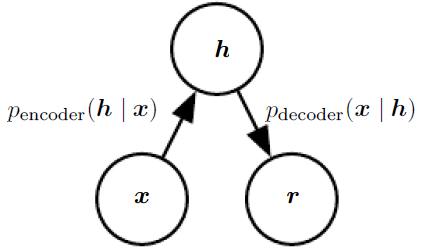
\includegraphics[width=2in]{fig/chap14/14_2.png} 
   \caption{随机自编码器结构图。其中编码器与解码器都不是简单的函数而是包含了一些噪声,这意味着他们的输出可以看作是从要给概率分布中抽样获得的,编码的分布为$p_{encoder(\bm{h}|\bm{x})}$,解码的分布为$p_{decoder}(\bm{x}|\bm{h})$。}
   \label{fig:14.2}
\end{figure}

任何隐变量模型$p_{model}(h,x)$都可以用来定义随机编码器
\begin{equation}
	p_{encoder}(h|x) = p_{model}(h|x)
\end{equation}
和随机解码器
\begin{equation}
	p_{decoder}(x|h) = p_{model}(x|h)
\end{equation}
通常来讲,编码器和解码器并不一定是同联合概率分布$p_{model}(x,h)$吻合的条件概率分布。Alain指出作为降噪自编码训练编码器和解码器能够使他们渐进兼容(在有足够容量和样本的情况下)。

\section{降噪自编码器}
\label{sec:14.5}
降噪自编码器是在给定的输入包含噪声的情况下训练以预测其未被干扰的输入的自编码器。

降噪自编码器额训练过程在图\ref{fig:14.3}中给出。我们介绍加噪处理$C(\hat{x}|x)$,其代表在给出训练样本$x$时的$\hat{x}$的条件概率分布。自编码器从训练样本对$(x,\hat{x})$中学习到\emph{重建分布}$p_{reconstruction}(x|\hat{x})$,过程如下:

1. 从训练样本中抽取一个样本$x$。

2. 从分布$C(\hat{x}|x)$中抽取带有噪声的样本$\hat{x}$。

3. 将$(x,\hat{x})$作为训练样本去预测自编码器的重建分布$p_{reconstruction}(x|\hat{x}) = p_{decoder}(x|h)$,其中,$\bm{h}$是编码器$f(\hat{x})$的输出,$p_{decoder}$一般是由解码器$g(\bm{h})$给出。

一般来讲,我们可以对负对数似然$-log p_{decoder}(x|h)$做基于梯度的近似最小化(如小批次梯度下降)。只要编码器是确定性的,降噪自编码器就是前馈神经网络,并且可以用其他前馈网络的训练方法进行训练。
\begin{figure}[htbp] %  figure placement: here, top, bottom, or page
   \centering
   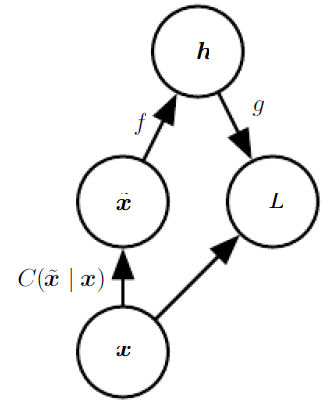
\includegraphics[width=2in]{fig/chap14/14_3.png} 
   \caption{降噪自编码器的损失计算图,即训练其使得能够从带噪声的样本$\hat{x}$中恢复出干净的样本$x$来。训练是通过最小化损失$L = -log p_{decoder}(x|h = f(\hat{x}))$得到的,其中$\hat{x}$是从加噪函数$C(\hat{x}|x)$得到的含有噪声版本的$x$。通常$p_{decoder}$是一个因子分布,其参数均值由前向网络$g$给出。}
   \label{fig:14.3}
\end{figure}

我们可以把降噪自编码器看作是针对下面期望的随机梯度下降:
\begin{equation}
 -\mathbb{E}_{x\sim \hat{p}_{data}(x)}\mathbb{E}_{\hat{x} \sim C(\hat{x}|x)}log p_{decoder}(x| h = f(\hat{x}))
\end{equation}
其中,$\hat{p}_{data}(x)$是训练样本分布。

\subsection{估算评分}
\label{sec:14.5.1}
评分估计是最大似然估计的一种替代方法。它能够通过促使模型在每一个样本点上同数据分布有一样的评分来给出概率分布的一个一致的估计值。此处,这个评分是一个特别的梯度域:
\begin{equation}
	\nabla_x log p(\bm{x})
\end{equation}
评分匹配在第\ref{sec:18.4}节中有更为细致的讲解。就当前对自编码器的讨论来讲,了解学习梯度域$log p_{data}$ 是学习$p_{data}$结构的一种方法就足够了。

降噪自编码的一个非常重要的性质就是他们的训练准则(用条件高斯$p(\bm{x}|\bm{h})$)使得自编码器学习到了一个计算数据分布评分的向量域$(g(f(x)) - x)$。请参考图\ref{fig:14.4}。
\begin{figure}[htbp] %  figure placement: here, top, bottom, or page
   \centering
   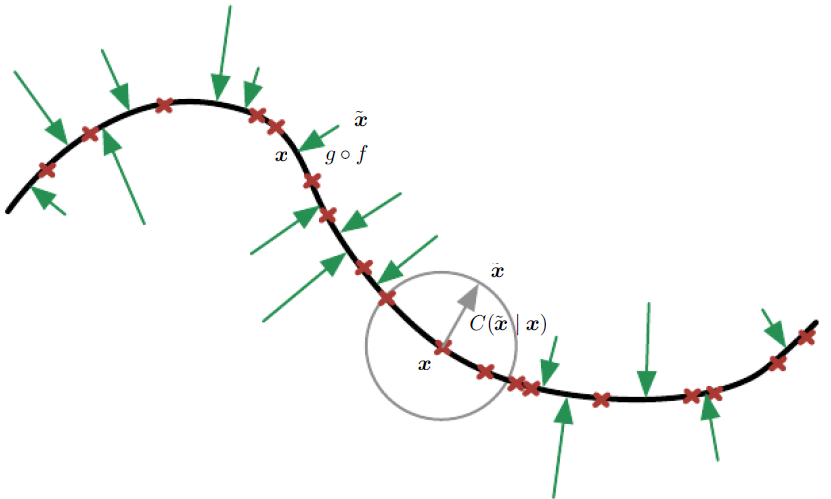
\includegraphics[width=4.5in]{fig/chap14/14_4.png} 
   \caption{降噪自编码器被训练用以将含噪数据$\hat{\bm{x}}$映射回原始数据$\bm{x}$。原始数据用红色X号表示,其处于黑色实线表示的一维流面上。加噪函数$C(\bm{\hat{x}},\bm{x})$用灰色圆圈表示其各向同性。灰色箭头表示了样本是如和从流面被引入噪声映射到别处的。当降噪自编码器被训练来降低均方误差$\|g(f(\hat{x})) -x \|^2$时,重建函数$g(f(\hat{x}))$计算了期望$\mathbb{E}_{x,\hat{x} \sim p_{data} C(\bm{\hat{x}}, \bm{x})}[\bm{x}|\bm{\hat{x}}]$。向量$g(f(\hat{\bm{x}})) - \hat{\bm{x}}$指向了流面上最近的点,这是因为$g(f(\hat{\bm{x}}))$估算的可能产生噪点$\bm{\hat{x}}$的纯净数据$\bm{x}$的重心。因此自编码器学习到了一个向量空间$g(f(\hat{\bm{x}})) - \bm{x}$,图中绿线所示。这个向量域用一系列乘数因子计算评分$\nabla x \log p_{data}(\bm{x})$,这些因子是重建均方误差的根值平均数。}
   \label{fig:14.4}
\end{figure}

用高斯噪声和均方差作为重建损失来训练一个特定的降噪自编码器(隐层为sigmoid单元,重建为线性单元)等效于训练一种特定的具有高斯可观察单元的称为RBM的无向图模型。这种模型将会在第\ref{SEC:20.5.1}节进行详细介绍;此处仅需知道他是一种能够提供明确函数$p_{model}(\bm{x};\bm{\theta})$的模型即可。当RBM被用\emph{降噪评分匹配}来进行训练的时候,其学习算法等同于和它对应的自编码器的降噪训练。给定特定的噪声值,泛化评分匹配并不是一个一致的估算;它其实恢复了一个模糊化的分布。但是,如果噪声水平接近于零,并且训练样本趋近于无穷,此时一致性又得到了恢复。降噪评分匹配在第\ref{sec:18.5}节有详细讨论。

RBM同自编码器还有其他的联系。评分匹配应用到RBM上产生的损失函数等同于重建误差加上一个同收缩自编码中的收缩项相似的正则化项。Bengio等人指出自编码器的导数为RBM的contrastive divergance计算提供了近似。

对于连续值$\bm{x}$,包含高斯噪声和重建分布的降噪标准为常规编码器和解码器的参数化评分计算提供了依据。这意味着生成编码-解码结构通过训练后可以被用来计算评分,训练用的均方误差标准为
\begin{equation}
	\|g(f(\bm{\hat{x}})) - \bm{x}\|^2
\end{equation}
以及噪声
\begin{equation}
	C(\hat{x} = \bm{\hat{x}} | \bm{x}) = \mathcal{N}(\bm{\hat{x}}; \mu = \bm{x}, \Sigma = \sigma^2I)
\end{equation}
其中,$\sigma^2$为噪声方差。关于具体如何运作,请参考图\ref{fig:14.5}。
\begin{figure}[htbp] %  figure placement: here, top, bottom, or page
   \centering
   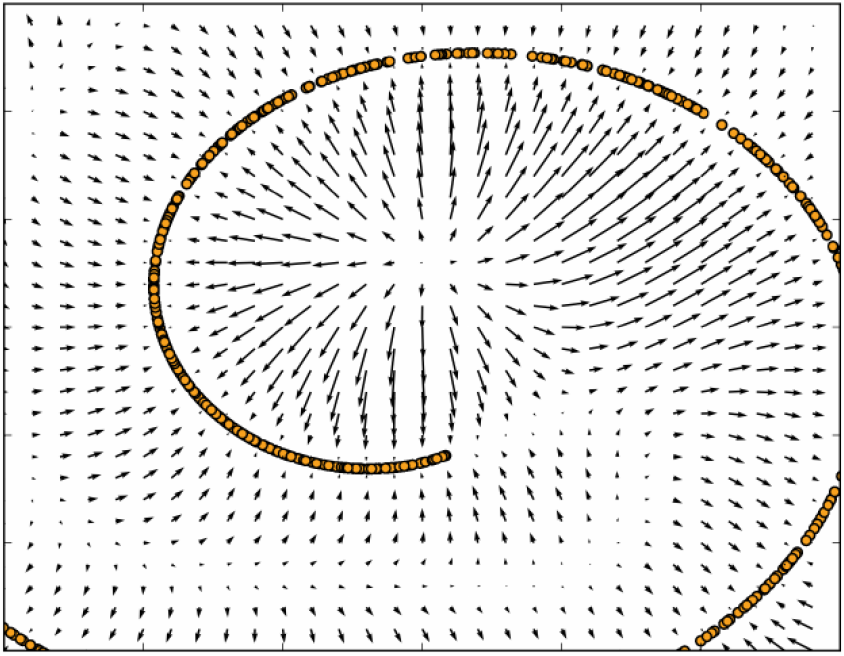
\includegraphics[width=4.5in]{fig/chap14/14_5.png} 
   \caption{降噪自编码器学习到的二维空间中的一维曲面流面附近的向量域。每一个箭头都与重建向量减去输入向量的值成一定比例并且箭头指向预测到的概率分布的较高概率值。向量域在估算的密度函数的极大值(在数据流面上)与极小值处取值为零。例如,螺旋的臂构成了相互连接的有局部极大值的一维流面。局部极小值在两个臂之间的区域的中间位置。当重建误差的模(以箭头的长度表示)较大的时候,意味着沿着箭头的方向移动的话概率值可以得到很大的提升,反之亦然。自编码器将这些低概率的点映射为高概率的重建值。在概率取得极大值的地方,箭头缩短,因为此时的重建值更加精确。}
   \label{fig:14.5}
\end{figure}

通常来讲,并没有任何保证说重建$g(f(x))$ 减去输入$\bm{x}$对应于任何方程的导数,更别提评分了。如此可以解释为什么早期的结果只能应对特定的参数,即$g(f(x)) - x$ 仅可以通过另一个方程的导数来获得。Kamyshanska通过定义一族浅层自编码器使$g(f(x)) - x$对族内所有成员都有对应的评分,如此进一步优化了Vincent的结果。

至此我们仅讨论了降噪自编码器是如何学习表示一个概率分布的。更一般来讲,我们可能会想用自编码器作为生成模型并从其分布中抽取样本。这些将在后面第\ref{sec:20.11}节讨论。

\subsubsection{历史回顾}
\label{sec:14.5.1.1}

\section{用自编码器进行流行学习}
\label{sec:14.6}

同其他很多机器学习方法一样,自编码器同样假设数据集中在一个低维流面或者一个这种流面的小集合上,详见\ref{sec:5.11.3}节。一些机器学习方法效果有限,尽管他们可能可以学习到一个在流面上正常的函数,但是对于不在流面上的输入,可能会产生不正常的表现。
自编码器进一步拓展了这种思想,并设法去学习流行的结构。

为了理解为什么自编码器能够有这样的效果,我们需要介绍流行的几个重要的特性。

其中一个很重要的特性是其\emph{正切平面}集合。对于一个d-维流面上的点$x$, 其切面是由能够张成流面上局部方向变化的d-维向量给出。如图\ref{fig:14.6}所示,这些局部方向指出了我们能如何对$x$在流面上进行无限小的位置改变。
\begin{figure}[htbp] %  figure placement: here, top, bottom, or page
   \centering
   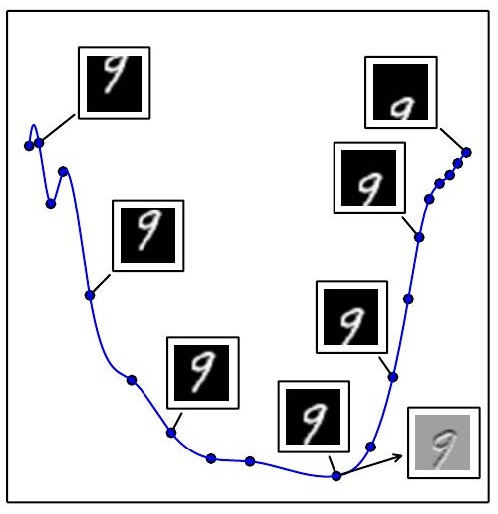
\includegraphics[width=4in]{fig/chap14/14_6.jpg} 
   \caption{超切平面概念示意图。这里我们给出一个784-维空间内的一维流面。我们选取MNIST数据集中的一幅784像素的图像,并沿着竖直方向移动它。这样的一组竖直移动数据定义了沿一维流面方向的坐标,并在图像空间中划出一条曲线。图中给出了在这个流面上的几个点。为了可视效果,我们用PCA把流面投影到了二维空间中。一个n维流面在任一点都有一个n维切面。切面在流面上的该点处完美贴合,并且与该点的表面平行。该切面定义了使得数据保持在流面上的可以移动的方向空间。图中的一维流面有一个单独的切线。我们在图中给出了一个切线示例,以及在图像空间中沿切线移动时所产生的变化。灰色的像素是在移动过程这个不发生变化的点,白色代表颜色变亮,黑色代表颜色加深。}
   \label{fig:14.6}
\end{figure}

所有的自编码器的训练过程是两个限定因素的折衷:

1. 学习一个训练样本$x$的特征表示$h$,使得$x$能够通过解码器从$h$中大致恢复出来。$x$是从训练样本抽取的这个事实使得问题有点儿麻烦,因为这意味着自编码器没有必要对与不在数据生成分布下的输入进行很好的重建。

2. 满足限定或者泛化惩罚。这个可以是结构上限定自编码器的容量的设定,或者是添加到重建误差后的一项泛化项。这些技术通常倾向于对于输入数据不敏感的解决方案。

显然,不管是从输入到输出的复制本身,或者是直接忽略输入,二者任何之一单独出现都没有太大作用。相反,二者同时出现,能够保证方法有效,因为他们迫使隐藏特征表示去捕获能够描述数据生成分布的内在结构。重要的一点就是自编码器可以只去表示重建训练数据所必须的那些变化。如果生成数据的分布本身集中在一个低维流面上,这诱使特征描述仅仅表现这个流面上的一个局部的坐标系统:即只有在$x$附近的与流面相切的变化可以联系到$h = f(x)$的改变上。所以,自编码器学到的从输入空间$x$到表示空间的映射,是一个仅仅对于在流面方向上的变化敏感但对于垂直于流面方向上的变化不敏感的映射。

图\ref{fig:14.7} 给出了一个一维的例子,该图表明通过限定重建函数对于数据点周围扰动的敏感性,我们的自编码器可以重建流面结构。
\begin{figure}[htbp] %  figure placement: here, top, bottom, or page
   \centering
   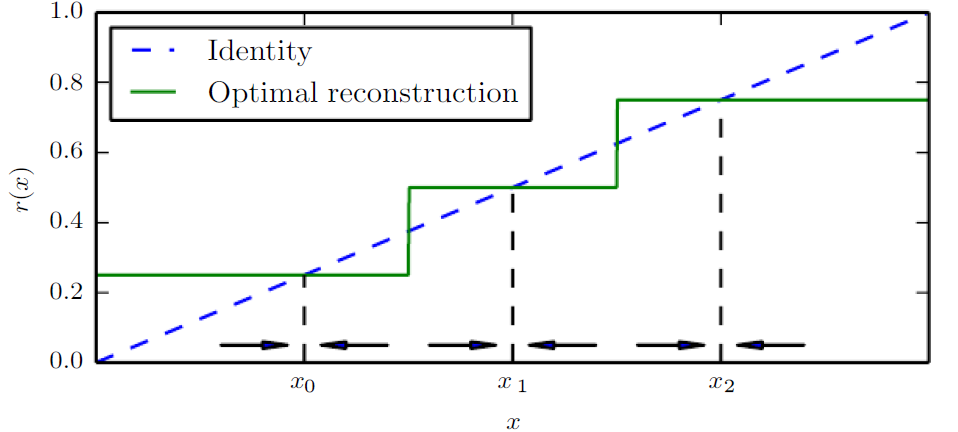
\includegraphics[width=4in]{fig/chap14/14_7.png} 
   \caption{如果自编码器学习到了一个能够对在数据点周围的扰动具有不变性的重建方程,则其学习到了数据本身的流行结构。图中给出的是0-维流面的流行结构。虚线表示用以重建的恒等函数。最有重建函数在有数据的地方同恒等函数重合。底部的箭头表示重建误差向量$r(x)-x$,在输入空间,这些箭头总是指向其最近的“流面”(在一维的情况下,是一个孤立点)。降噪自编码器直接设法使重建函数$r(x)$的偏导数在数据点周围尽量小。收缩自编码器对于编码器进行了同样的操作。尽管$r(x)$的导数在数据点周围尽量小,在不同数据点之间,它可以变得很大。数据点之间的空间同流面之间的区域直接相关,在这些地方,重建函数的导数必须很大,才能将被破坏的点重新映射回流面上。}
   \label{fig:14.7}
\end{figure}

为了更好的理解为什么自编码器可以进行流行学习,我们有必要将其与其他方法进行比较 。对于流行的特性最常用的研究方法是点在流面上或者流面附近的\emph{特征表示}。对于某个样本的特征表示也被称作其嵌入。特征表示通常用一个低维的向量来表示,即比作为一个低维子集存在的流面的原始外部空间的维数要低。一些算法直接对每一个训练样本学习一个嵌入表示(如下面导论到的非参数流行学习方法),与此同时,其他的一些方法则设法学习到一个更为通用的映射,该映射将周围空间(输入空间)映射到嵌入空间。有时这种映射被叫做自编码器或者表示方程式。 

流行学习通常关注于非监督学习的方法来得到这些流面。早期的大部分学习流面的研究集中在基于最近邻图模型的非参数方法上。在图模型中,每个样本表示为一个节点,并通过边将最近邻的样本连接起来。如图\ref{fig:14.8}所示,这些方法将每个节点表示为切平面,这些切平面描述了样本同其邻域样本的变化方向。
\begin{figure}[htbp] %  figure placement: here, top, bottom, or page
   \centering
   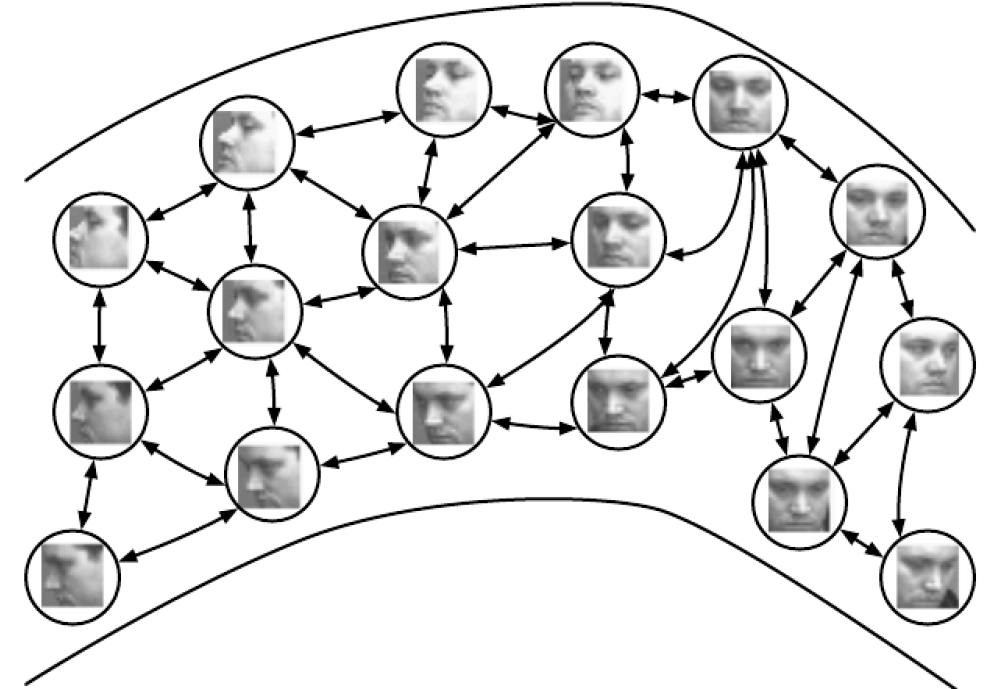
\includegraphics[width=4in]{fig/chap14/14_8.png} 
   \caption{非参数流行学习方法构建了一个最近邻图模型,其中,节点表示训练样本,有向边表明最近邻关系。如此,通过各种不同的方法可以得到切平面以及与其相对应的邻域图模型,此外,还有一个将每一个样本同一个实值向量或嵌入对应的坐标系统。如此我们可以通过一定的改动使特征表示适应新的样本。只要样本数量足够大能够覆盖流面的弯曲与褶皱,这些方法都可以很好的工作。图片来源为QMUL多视人脸数据库。}
   \label{fig:14.8}
\end{figure}

我们之后可通过优化算法或者求解线性系统来获取一个全局坐标系统。图\ref{fig:14.9}给出了一个流面视如何平铺成大量的局部线性类高斯碎片的(或者叫做圆饼,因为高斯函数在切线方向是平坦的)。
\begin{figure}[htbp] %  figure placement: here, top, bottom, or page
   \centering
   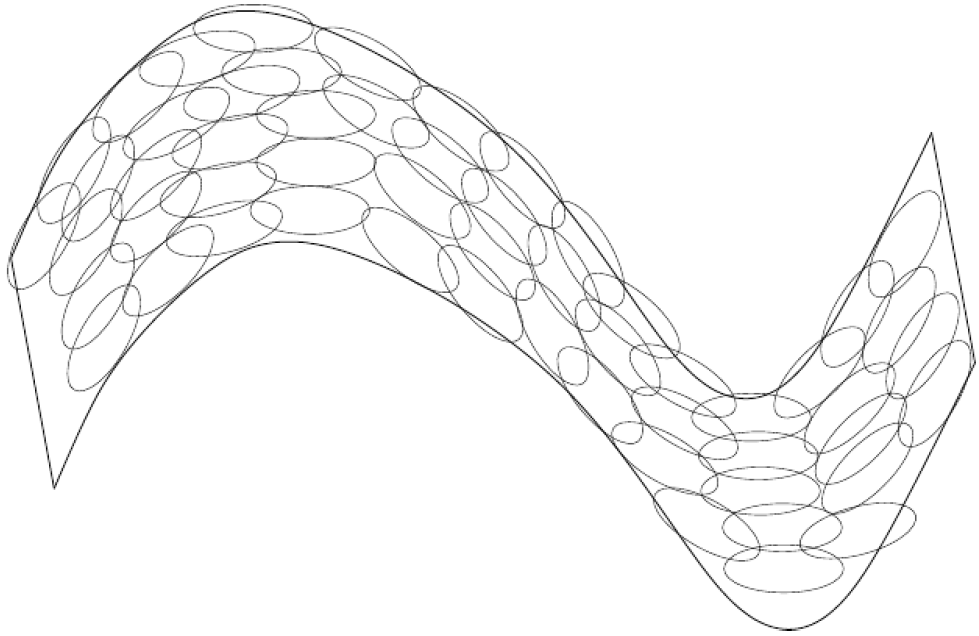
\includegraphics[width=4in]{fig/chap14/14_9.png} 
   \caption{如果切平面(参考图\ref{fig:14.6})在处处都是已知的,则他们可以平铺成一个全局的坐标系统或者密度方程。每一个局部分块都可以被看成是一个局部的欧氏坐标系统或者局部扁平高斯或者圆盘,他们在垂直于圆盘的方向变化很小,在定义圆盘坐标系统的方向上变化很大。这样的一些高斯函数组合成了在流面高斯窗算法或者其基于非局部神经网络的变种中的一个预测密度函数。}
   \label{fig:14.9}
\end{figure}

但是,用这些局部非参数的方法在进行流行学习的时候有一个基本的难题:如果流面本身非常不平整(有许多峰值、低谷、褶皱),我们可能需要大量的样本来覆盖这些变量,从而降低了对未知样本的泛化能力。事实上,这些方法仅仅能够通过邻域信息的插值来泛化流面的形状。不幸的是,在人工智能问题中涉及到的流行往往具有非常复杂的结构,很难从局部插值中获取所有信息。比如说图\ref{fig:14.6}中的通过平移变换产生的流面,如果我们仅仅观察输入向量的一个坐标$x_i$的话,当图像移动时,我们可以看到,每当图像在遇到灰度的峰值或者低谷的时候,我们的坐标就会遇到一个峰值或者低谷。换言之,待处理图像的灰度明暗的复杂度决定了对于像进行简单的平移操作产生的流面的复杂度。这些促使了通过分布式描述和深度学习进行流行结构学习的需求。
%%%%%%%%%%%%%%%%%%%%%%%%%%%%%%%%%%%%%%%%%%%%%%%%%%%%%%%%%
%%%%%%%%%%%%%%%%%%%author:Euniceu%%%%%%%%%%%%%%%%%%%%%%%%
%%%%%%%%%%%%%%%%%%%part:14.7-14.9%%%%%%%%%%%%%%%%%%%%%%%%
%%%%%%%%%%%%%%%%%%%%%%%%%%%%%%%%%%%%%%%%%%%%%%%%%%%%%%%%%

\section{14.7}

%%%%%%%%%%%%%%%%%%%%%%%%%%%%%%%%%%%%%%%%%%%%%%%%%%%%%%%%%
%%%%%%%%%%%%%%%%%%%  author:tangzhenyu %%%%%%%%%%%%%%%%%%
%%%%%%%%%%%%%%%%%%%  part:15.0-15.3    %%%%%%%%%%%%%%%%%%
%%%%%%%%%%%%%%%%%%%%%%%%%%%%%%%%%%%%%%%%%%%%%%%%%%%%%%%%%

\chapter{表征学习}
\label{chap:15}
\section{15.1}
\label{sec:15.1}
%%%%%%%%%%%%%%%%%%%%%%%%%%%%%%%%%%%%%%%%%%%%%%%%%%%%%%%%%
%%%%%%%%%%%%%%%%%  author:chongruo  %%%%%%%%%%%%%%%%%%%%%
%%%%%%%%%%%%%%%%%  part:15.4-15.6   %%%%%%%%%%%%%%%%%%%%%
%%%%%%%%%%%%%%%%%%%%%%%%%%%%%%%%%%%%%%%%%%%%%%%%%%%%%%%%%

\section{15.4}

\chapter{深度学习的结构化概率模型}
\label{chap:16}
%%%%%%%%%%%%%%%%%%%%%%%%%%%%%%%%%%%%%%%%%%%%%%%%%%%%%%%%%
%%%%%%%%%%%%%%% author: YisenWang   %%%%%%%%%%%%%%%%%%%%%%%%%%%
%%%%%%%%%%%%%%% part:16.0-16.2.5 %%%%%%%%%%%%%%%%%%
%%%%%%%%%%%%%%%%%%%%%%%%%%%%%%%%%%%%%%%%%%%%%%%%%%%%%%%%%
%%%%%%%%%%%%%%%%%%%%%%%%%%%%%%%%%%%%%%%%%%%%%%%%%%%%%%%%%
%%%%%%%%%%%%%%% author:heailong2013 %%%%%%%%%%%%%%%%%%%%%%%%%%%
%%%%%%%%%%%%%%% part: 16.2.6-16.6       %%%%%%%%%%%%%%%%%%%%%%%%%%%
%%%%%%%%%%%%%%%%%%%%%%%%%%%%%%%%%%%%%%%%%%%%%%%%%%%%%%%%%

\chapter{蒙特卡洛方法}
\label{chap:17}
%%%%%%%%%%%%%%%%%%%%%%%%%%%%%%%%%%%%%%%%%%%%%%%%%%%%%%%%%
%%%%%%%%%%%%%%%%%%% author:kiseliu  %%%%%%%%%%%%%%%%%%%%%
%%%%%%%%%%%%%%%%%%% part17.0-17.3   %%%%%%%%%%%%%%%%%%%%%
%%%%%%%%%%%%%%%%%%%%%%%%%%%%%%%%%%%%%%%%%%%%%%%%%%%%%%%%%
\section{吉布斯采样}
\label{sec:17.4}

到目前为止,本章已经介绍了如何通过迭代更新$x\rightarrow x' \sim T (x'|x) $在概率分布$q(x)$上采样的方法.
但是,还没有说明怎样确保$q(x)$是有效的概率分布.
本书主要考虑两种基本方法.第一种方法根据给定的通过学习得到的$p_{model}$推导出$T$,下文将会详细介绍从EBMs(energy-based model)采样的例子.
第二种方法是直接参数化$T$并学习,使其平稳分布可以隐式地定义$p_{model}$的兴趣点.
第二种方法的例子将在章节"\textcolor{red}{20.12}"和"\textcolor{red}{20.13}"阐述.

在深度学习中,通常使用马尔科夫链从以基于能量的模型定义的概率分布$p_{model}$中采样.
此例中,马尔科夫链所需的$q(x)$就是$p_{model}$.
为得到满足需求的$q(x)$,必须选择合适的$T(x'|x)$.

为了构建马尔科夫链,一种概念上简单有效的方法就是使用\textit{吉布斯采样}从$p_{model}$中采样.
在吉布斯采样中,通过选择一个变量$x_i$实现从$T(x'|x)$中采样,$x_i$的选择方法取决于它在基于能量模型结构的无向图$\mathcal{G}$上的邻居变量.
只要给定的所有邻居节点都条件独立,也可以同时对多个变量采样.
在$16.7.1$中的RBM(受限玻尔兹曼机)例子中,RBM的所有隐含层单元可以被同时采样,是因为他们都条件独立于其他的给定可视层单元.
同样的,因为对于给定的隐含层单元,所有的可视层单元都是条件独立的,因此所有的可视层单元也可以同时被采样.
以这种方式同时更新多个变量的吉布斯采样方法,被称为块吉布斯(block gibbs)采样.

从$p_{model}$中采样来设计马尔科夫链的代替方法是可行的.例如,Metropolis-Hastings算法就广泛应用于其他学科领域.
在深度学习领域实现无向建模,除吉布斯采样外很少使用其他方法.
改进采样技术是一个潜在的研究领域.

\chapter{直面配分函数}
\label{chap:18}
% Partition Function 配分函数的定义见 wiki:https://www.wikiwand.com/zh/%E9%85%8D%E5%88%86%E5%87%BD%E6%95%B0

%%%%%%%%%%%%%%%%%%%%%%%%%%%%%%%%%%%%%%%%%%%%%%%%%%%%%%%%%
%%%%%%%%%%%%%%%%%%% author:quxiaofeng %%%%%%%%%%%%%%%%%%%
%%%%%%%%%%%%%%%%%%%%%%%%%%%%%%%%%%%%%%%%%%%%%%%%%%%%%%%%%

如 \consider{16.2.2 节}中所见,很多概率模型(一般称为无向图模型)是用\consider{非标准化(unnormalized)}的概率分布 \(\widetilde{p}(\bm{x};\bm{\theta})\) 定义的。必须要用配分函数 \(Z(\bm{\theta})\) \footnote{译者注:配分函数(Partition Function)的定义见 wiki:\url{https://www.wikipedia.org/zh/\%E9\%85\%8D\%E5\%88\%86\%E5\%87\%BD\%E6\%95\%B0}} 去除 \(\widetilde{p}\) 才能得到有效的概率分布:
\begin{equation}
    p(\bm{x};\bm{\theta})
    = \frac{1}{Z(\bm{\theta})}\widetilde{p}(\bm{x};\bm{\theta}).
\end{equation}

配分函数是\consider{非标准化}概率对于所有状态的积分(连续变量)或和(离散变量): 
\begin{equation}
    \int\widetilde{p}(\bm{x})d\bm{x}
\end{equation}
 或者
 \begin{equation}
     \sum_{\bm{x}}\widetilde{p}(\bm{x}).
 \end{equation}

这个运算对于很多常用模型来说是\consider{不可解的(intractable)}。

如\consider{20 章}所见,有些深度学习模型在设计上是有可解标准化常量的,或者设计为无需计算 \(p(\bm{x})\)。但其它的模型就需要直接面对不可解配分函数的问题了。本章我们讨论训练和评估具有不可解配分函数的模型的方法。

\section{对数似然梯度}
\label{sec:18.1}

使用最大似然法学习无向模型的难点在于配分函数有参数依赖。相对参数的对数似然梯度具有与配分函数梯度相关项:
\begin{equation}
    \nabla_{\bm{\theta}}\log{p(\bm{x};\bm{\theta})}
    = \nabla_{\bm{\theta}}\log{\widetilde{p}(\bm{x};\bm{\theta})}
    - \nabla_{\bm{\theta}}\log{Z(\bm{\theta})}.
\end{equation}

这里就是著名的\consider{正相(positive phase)学习与负相(negative phase)学习}分解的产生。

对于大多数我们所关心的无向图模型,负相比较难。没有隐变量或者隐变量\consider{交互,连接}比较少的模型一般具有可解的正相。具有简单正相、复杂负相的模型的最基础的例子就是 RBM。给定可见单元,RBM 的隐单元之间条件独立。正相复杂、隐变量之间交互复杂的例子,主要集中于第 19 章。本章关注负相的复杂度。

再仔细观察一下\(\log Z\)的梯度:
\begin{align}
    & \nabla_\theta \log{Z}                                \\
    & = \frac{\nabla_\theta Z}{Z}                          \\
    & = \frac{\nabla_\theta\sum_x\widetilde{p}(\bm{x})}{Z} \\
    & = \frac{\sum_x\nabla_\theta\widetilde{p}(\bm{x})}{Z}.
\end{align}

若模型对所有 \(\bm{x}\) 都有 \(p(\bm{x})>0\),则可用 \(exp(\log\widetilde{p}(\bm{x}))\) 代换 \(\widetilde{p}(\bm{x})\):
\begin{align}
& \frac{\sum_x\nabla_\theta\exp(
    \log{\widetilde{p}(\bm{x})})}{Z}             \\
& = \frac{\sum_x\exp(\log{\widetilde{p}(\bm{x})})
    \nabla_\theta\log{\widetilde{p}(\bm{x})}}{Z} \\
& = \frac{\sum_x\widetilde{p}(\bm{x})
    \nabla_\theta\log\widetilde{p}(\bm{x})}{Z}   \\
& = \sum_{\bm{x}}p(\bm{x})
    \nabla_\theta\log\widetilde{p}(\bm{x})       \\
& = \mathbb{E}_{x\sim{}p(\bm{x})}
    \nabla_\theta\log\widetilde{p}(\bm{x}).
\end{align}

这个推导利用了离散 \(\bm{x}\) 的求和。对于连续的 \(\bm{x}\),利用积分也可以得到相似的结果。在连续版的推导中,可以使用积分号下的莱布尼茨法则得到同样的结果
\begin{equation}
    \nabla_{\bm{\theta}}\int\widetilde{p}(\bm{x})d\bm{x}
    = \int\nabla_{\bm\theta}\widetilde{p}(\bm{x})d\bm{x}.
\end{equation}
这一等同的结果只是在 \( \widetilde{p} \) 和 \( \nabla_{\bm\theta}\widetilde{p}(\bm{x})d\bm{x} \) 满足一定的正则化条件时成立。根据测度论,需要满足如下条件:(i) 非正态分布\( \widetilde{p} \) 对每一个 \(\bm{\theta}\)都是 \(\bm{x}\) 的勒贝格可积函数;(ii) 梯度 \( \nabla_{\bm\theta}\widetilde{p}(\bm{x}) \) 必须对所有 \(\bm\theta\) 和几乎所有 \(\bm x\) 都存在;(iii) 必须存在一个 \( \nabla_{\bm\theta}\widetilde{p}(\bm{x}) \) \consider{的可积确界函数} \(R({\bm x})\),使得 \(\max_i|\frac{\partial}{\partial \theta_i}\widetilde{p}(\bm{x})| \leq R(\bm{x}) \) 对所有 \(\bm\theta\) 和几乎所有 \(\bm x\) 都成立。幸好,常见机器学习模型都具有这些性质。

这种一致性
\begin{equation}\label{eqn:18.15}
    \nabla_{\bm{x}}\log{}Z
    = \mathbb{E}_{\bm{x}\sim{}p(\bm{x})}
    \nabla_{\bm{\theta}}\log\widetilde{p}(\bm{x})
\end{equation}
是蒙特卡洛方法经过适当改进后可以近似地求得配分函数可解模型的最大似然的基础。

学习无向图模型的蒙特卡洛方法为我们提供了直观的框架,可以同时考虑正相和负相。正相,根据从数据中提取的 \(\bm x\) 提高 \(\log\widetilde{p}(\bm x)\)。负相,根据模型分布降低配分函数降低 \(\log\widetilde{p}(\bm x)\)。

在深度学习文献中,一般把 \(\log\widetilde{p}\) \consider{参数化(parameterize)}为能量函数\consider{(公式 16.7)}。
这里,我们可以把正相解释为压低训练样本的能量;把负相解释为抬高模型中央本的能量,参见图~\ref{fig:18.1}。

\section{随机最大似然和对比分歧}
\label{sec:18.2}

\begin{algorithm}
\DontPrintSemicolon
设置 \(\epsilon\),步长,应设为较小正数。\;
设置 \(k\),吉布斯(Gibbs)步长,设置时应考虑为预热(burn in)提供冗余,设置一个较大的值。在一个小图像块上训练 RBM 大约可以设为 100。\;
\While{未收敛}{
    从训练集中抽样一个包含 \(m\) 个样本 \(\{\bm{x}^{(1)},\ldots,\bm{x}^{(m)}\}\) 的小批(minibatch)\;
    \(\bm{g} \longleftarrow \frac{1}{m}\sum^m_{i=1}
        \nabla_{\bm{\theta}}\log\widetilde{p}(\bm{x}^{(i)};\bm{\theta})\).\;
    用随机数初始化一组 \(m\) 个样本 \(\{\widetilde{\bm{x}}^{(1)},\ldots,\widetilde{\bm{x}}^{(m)}\}\)(可以使用均匀分布或正态分布,或者也可以使用与目标边缘分布相匹配的分布)。\;
    \For{\(i=1\) to \(k\)}{
        \For{\(j=1\) to \(m\)}{
            \(\widetilde{\bm{x}}^{(j)} 
            \longleftarrow \text{吉布斯更新}(\widetilde{\bm{x}}^{(j)}).\)\;
        }
    }
    \(\bm{g} \longleftarrow
        \bm{g} - \frac{1}{m}\sum^m_{i=1}
        \nabla_{\bm{\theta}}\log\widetilde{p}(\bm{x}^{(i)};\bm{\theta})\).\;
    \(\bm{\theta} \longleftarrow
        \bm{\theta} + \epsilon\bm{g}\)\;
}
\caption{一个朴素的蒙特卡洛马尔科夫链算法(MCMC)算法。利用梯度上升来计算带有可解配分函数的最大对数似然。\label{alg:18.1}}
\end{algorithm}

实现公式~\ref{eqn:18.15} 的一个简单方法,是每次需要梯度的时候,预热一组随机初始化的马尔可夫链,再进行计算。使用随机梯度下降进行学习时,每次计算梯度马尔可夫链都要预热。此方法的训练过程如算法~\ref{alg:18.1} 所示。该方法在内循环中预热马尔可夫链,运算过于复杂,但为更为实际的算法提供了基准。

MCMC 求最大似然,可以看做是在两种力量中取得平衡。一方面,产生数据的地方,推高模型分布;另一方面,模型采样产生的地方压低模型分布。图~\ref{fig:18.1} 所示即为此过程。两种力量分别对应于最大化 \(\log\widetilde{p}\) 和最小化 \(\log Z\)。有几种可行的近似负相的方法。但这些近似方法都可以理解为降低负相计算复杂性的同时,在一些错误的位置压低分布。

\begin{figure}[htbp] %  figure placement: here, top, bottom, or page
   \centering
   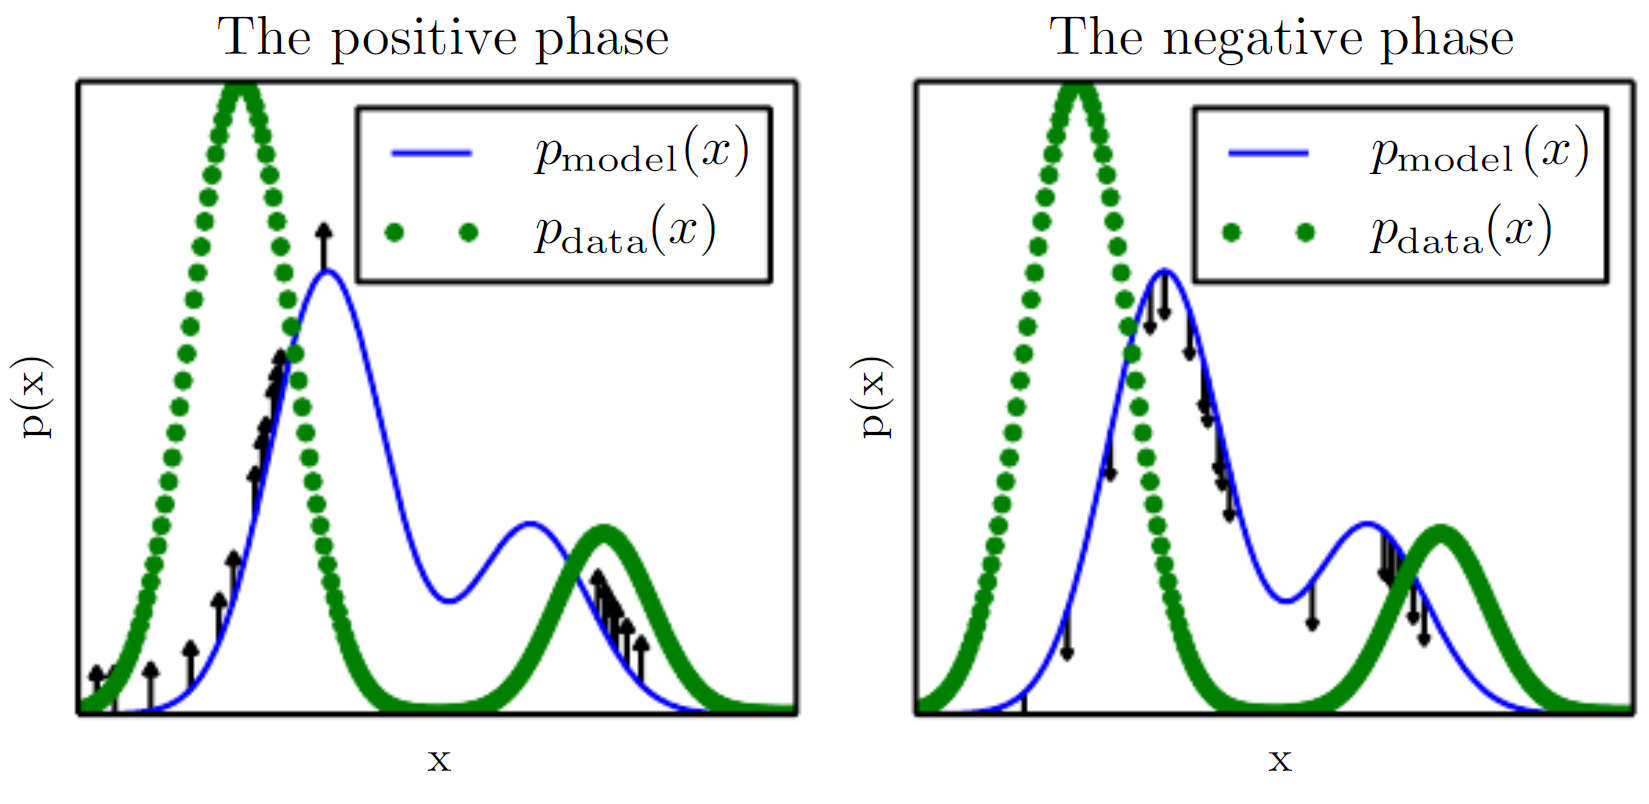
\includegraphics[width=\textwidth]{fig/chap18/18_1.png} 
   \caption{算法~\ref{alg:18.1} 的``正相''和``负相''。(左)正相时,我们从数据分布中采样一些点,然后推高非标准化的概率。数据中更有可能的点会推高得更多。(右)负相时,我们从模型中采样一些点,然后压低它们的非标准化概率。负相抵消了正相为非标准化概率在每一个位置都简单增加一个巨大常量的倾向。当数据分布和模型分布相等时,正相与负相在一点上推高和压低的几率相等。这时,梯度(的期望)就没有了,训练必然终止。}
   \label{fig:18.1}
\end{figure}

负相需要从模型分布中提取样本,这一过程开始理解为从模型中找一些非常有信心的点。
因为负相降低这些点的概率,一般认为这些是模型对世界的错误认知。
文献中一般称之为\consider{``幻象(Hallucinations)''}或\consider{``神奇粒子(Fantasy particles)''}。
其实,还真的曾有人提出负相可能是人类和其它动物做梦的原因\consider{(Circk and Mitchison, 1983)}。
其主要概念是说,大脑维护一个对于整个世界的概率模型。清醒时,当真实事件发生时,遵从 \(\log\widetilde{p}\) 的梯度;睡眠时,遵从 \(\log\widetilde{p}\) 的负梯度最小化 \(\log Z\),同时体验的则是当前模型的采样。
这个假说可以很好地解说正相和负相,他们之间的关系及其在算法中的作用,但并未被神经科学实验所证实。
机器学习模型中,经常要同时使用正相与负相,而不是像清醒与快速动眼睡眠一样分时进行。
如 \consider{19.5} 节所示,其它机器学习算法因为其它原因从模型分布中抽取样本,也可以算作睡眠时的梦境。

根据对于正相和负相学习理解,我们可以设计一个比算法~\ref{alg:18.1} 简单一点的方法。朴素 MCMC 算法主要的复杂度在每次循环中都需要用随机初始化预热马尔可夫链。一个很自然的解决方法是用一个与模型分布很接近的分布来初始化马尔可夫链,这样预热就不需要那么多步骤。

对比分歧(Contrastive Divergence,简称为 CD 或 CD-k,即 k 步吉布斯对比分歧)算法,用数据分布中的采样来初始化每步的马尔可夫链。\consider{(Hinton,2000,2010)}
从数据分布中采样,是 0 成本的,因为数据已经在数据集里准备好了。
一开始,数据分布与模型分布相差很远,负相不会很准确。
所幸,正相还是准确的,还是会增加数据的模型概率。
给与正相一定时间发挥作用之后,模型分布就会与数据分布相接近,负相就慢慢变得准确了。

\begin{algorithm}
\DontPrintSemicolon
设置 \(\epsilon\),步长,应设为较小正数。\;
设置 \(k\),吉布斯(Gibbs)步长,设置时,应考虑马尔可夫链从 \(p_{data}\) 中初始化时,需要从 \(p(\bm{x};\bm{\theta})\)中采样,设置为一个较大的值。在一个小图像块上训练 RBM 大约可以设为 1-20。\;
\While{未收敛}{
    从训练集中抽样一个包含 \(m\) 个样本 \(\{\bm{x}^{(1)},\ldots,\bm{x}^{(m)}\}\) 的小批(minibatch)\;
    \(\bm{g} \longleftarrow \frac{1}{m}\sum^m_{i=1}
        \nabla_{\bm{\theta}}\log\widetilde{p}(\bm{x}^{(i)};\bm{\theta})\).\;
    \For{\(i=1\) to \(m\)}{
        \(\widetilde{\bm{x}}^{(1)} \longleftarrow \bm{x}^{(i)}.\)\;
    }
    \For{\(i=1\) to \(k\)}{
        \For{\(j=1\) to \(m\)}{
            \(\widetilde{\bm{x}}^{(j)} 
            \longleftarrow \text{吉布斯更新}(\widetilde{\bm{x}}^{(j)}).\)\;
        }
    }
    \(\bm{g} \longleftarrow
        \bm{g} - \frac{1}{m}\sum^m_{i=1}
        \nabla_{\bm{\theta}}\log\widetilde{p}(\bm{x}^{(i)};\bm{\theta})\).\;
    \(\bm{\theta} \longleftarrow
        \bm{\theta} + \epsilon\bm{g}.\)\;
}
\caption{对比分歧算法。利用梯度上升进行优化。\label{alg:18.2}}
\end{algorithm}

\begin{figure}[htbp] %  figure placement: here, top, bottom, or page
   \centering
   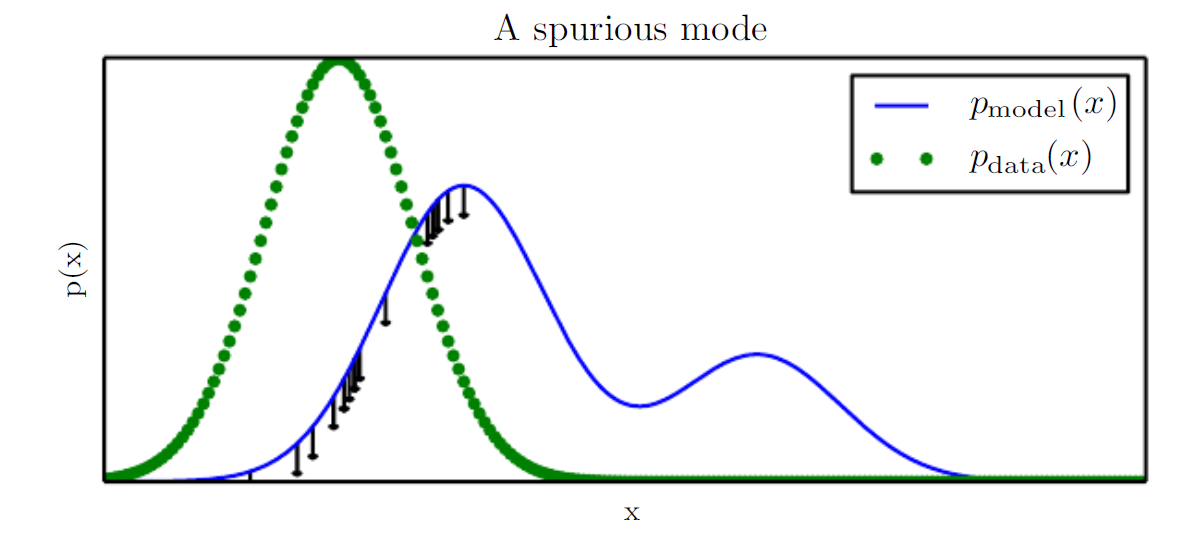
\includegraphics[width=\textwidth]{fig/chap18/18_2.png} 
   \caption{一个对比分歧算法(算法~\ref{alg:18.2})的负相无法抑制伪模式的例子。
   伪模式,是模型分布中存在,而数据分布中没有的模式。
   因为对比分歧从数据点中初始化它的马尔可夫链,且只跑几步马尔可夫链,不太有机会访问到模型上与数据点相距较远的模式。
   这意味着,在从模型上进行采样时会采集到不像数据的样本。
   这也意味着,模型在这些模式上浪费了概率,在正确的模式上投入高概率就很难实现了。
   出于便于可视化的考虑,图中使用了一种简化了的距离,伪模式与正确的模式在实数轴 \(\mathfrak{R}\)上相距较远。
   这对应的是在实数轴 \(\mathcal{R} \) 上只有一个单独变量 x 且只做局部运动的马尔可夫链。
   大多数深度概率模型,其马尔可夫链是基于吉布斯采样的,其对每一个单独的变量都可以做非局部的运动,只是不能同时移动所有的变量。
   这时,其实修改模式之间的距离度量,不用欧式距离会比较好。
   但高维空间中距离度量的修改,很难在二维图表中演示。}
   \label{fig:18.2}
\end{figure}

当然,对比分歧(CD)也是正确负相的一个近似算法。
CD 不能正确地实现负相的主要原因是抑制高概率的区域与训练样本相差太远。
在模型中高概率,在数据生成的分布中低概率的区域被称为\consider{``伪模式(Spurious Modes)''}。
图~\ref{fig:18.2} 展示了为什么会出现伪模式。
基本原因,是除非 k 非常大,模型分布中与数据分布相差较远的模式,根本不会被在训练点初始化的马尔可夫链访问到。

\consider{Carreira-Perpi\~nan and Hinton (2005)} 用实验演示了 CD 估计量对于 RBM 和完全可视玻尔兹曼机是有偏的。
实验中所收敛的点与最大似然估计量不同。
他们认为 CD 的偏置很小,作为一种低运算需求的算法,可以用来初始化模型,稍后再用原为复杂的 MCMC 方法微调。
\consider{Bengio and Delalleau (2009)} 发现 CD 解释成 MCMC 算法更新梯度时抛弃了最小的一些项。
这解释了为什么会有偏。



\section{伪概率}
\label{sec:18.3}

\section{评分比对和比率比对}
\label{sec:18.4}

\section{评分比对的降噪}
\label{sec:18.5}

\section{噪声抑制期望}
\label{sec:18.6}

\section{配分函数期望}
\label{sec:18.7}

\subsection{基于退火算法的重要性采样}
\label{sec:18.7.1}

\subsection{桥采样}
\label{sec:18.7.2}




\chapter{近似推理}
\label{chap:19}
%%%%%%%%%%%%%%%%%%%%%%%%%%%%%%%%%%%%%%%%%%%%%%%%%%%%%%%%%
%%%%%%%%%%%%%%%%% author:caigaojiang@gmail.com %%%%%%%%%%
%%%%%%%%%%%%%%%%%%%%%%%%%%%%%%%%%%%%%%%%%%%%%%%%%%%%%%%%%
\chapter{深度生成式模型}
\label{chap:20}

%%%%%%%%%%%%%%%%%%%%%%%%%%%%%%%%%%%%%%%%%%%%%%%%%%%%%%%%%
%%%%%%%%%%%%%%%%% author:Bruno-bai %%%%%%%%%%%%%%%%%%%%%%
%%%%%%%%%%%%%%%%%%%%%%%%%%%%%%%%%%%%%%%%%%%%%%%%%%%%%%%%%



\end{document}